%%%%%%%%%%%%%%%%%%%%%%%%%%%%%%%%%%%%%%%%%%%%%%%%%%%%%%%%%%%%%%%%%%%%%%%%%%%%%%%%
% Preámbulo                                                                    %
%%%%%%%%%%%%%%%%%%%%%%%%%%%%%%%%%%%%%%%%%%%%%%%%%%%%%%%%%%%%%%%%%%%%%%%%%%%%%%%%

\documentclass[11pt,a4paper,titlepage,oneside]{report}

%%% RELACIÓN DE VARIABLES A PERSONALIZAR %%%
\def\lingua{esp} 
\def\nome{Andrea Liñares Castro}                             
\def\nomedirectorA{Fernando Silva Coira}             
\def\nomedirectorB{Ángel Fernández Formoso}             % duplica esta liña máis veces se o precisas, cambiando
                                                     % a letra final (A, B, C, D...): úsanse na portada.tex
\def\titulo{Modernización del módulo Report Service en la plataforma BIC para el cliente AESLA} 
\def\titulacion{gei}
\def\mencion{SISTEMAS DE INFORMACIÓN}

%\def\renomearcadros{si} % descomenta esta liña se redactas a memoria en español e prefires que
                         % os "cuadros" e o "índice de cuadros" se renomeen
                         % a "tablas" e "índice de tablas" respectivamente

\usepackage{estilo_tfg}
\usepackage{enumitem}

% Lista de paquetes potencialmente interesantes (uso baixo demanda)

% \usepackage{alltt}       % proporciona o entorno alltt, semellante a verbatim pero que respecta comandos
% \usepackage{enumitem}    % permite personalizar os entornos de lista
% \usepackage{eurofont}    % proporciona o comando \euro
\usepackage{float}       % permite máis opcións para controlar obxectos flotantes (táboas, figuras)
% \usepackage{hhline}      % permite personalizar as liñas horizontais en arrays e táboas
  \usepackage{longtable}   % permite construir táboas que ocupan máis dunha páxina
% \usepackage{lscape}      % permite colocar partes do documento en orientación apaisada
% \usepackage{moreverb}    % permite personalizar o entorno verbatim
% \usepackage{multirow}    % permite crear celdas que ocupan varias filas da mesma táboa
% \usepackage{pdfpages}    % permite insertar ficheiros en PDF no documento
% \usepackage{rotating}    % permite diferentes tipos de rotacións para figuras e táboas
% \usepackage{subcaption}  % permite a inclusión de varias subfiguras nunha figura
% \usepackage{tabu}        % permite táboas flexibles
\usepackage{tabularx}    % permite táboas con columnas de anchura determinada
\usepackage{graphicx}
\usepackage{booktabs}
\usepackage{ragged2e}
\usepackage{pgfgantt}
\usepackage{tikz}
\usetikzlibrary{positioning}
\usepackage{xcolor}
\graphicspath{{img/}}

\usepackage[acronym]{glossaries}
\makeglossaries

%%%%%%%%%%%%%%%%%%%%%%%%%%%%%%%%%%%%%%%%%%%%%%%%%%%%%%%%%%%%%%%%%%%%%%%%%%%%%%%%
% Corpo                                                                        %
%%%%%%%%%%%%%%%%%%%%%%%%%%%%%%%%%%%%%%%%%%%%%%%%%%%%%%%%%%%%%%%%%%%%%%%%%%%%%%%%

\begin{document}

 %%%%%%%%%%%%%%%%%%%%%%%%%%%%%%%%%%%%%%%%
 % Preliminares do documento            %
 %%%%%%%%%%%%%%%%%%%%%%%%%%%%%%%%%%%%%%%%

 \include{portada/portada}
 \dedicatoria{A GBTEC Software AG, por la oportunidad de crecer y aprender en un entorno profesional.} 
 \paxinaenbranco
 \begin{agradecementos}
 Quiero agradecer a GBTEC Software AG, y especialmente a Ángel, mi tutor, y a
 Ana, mi compañera, la oportunidad de realizar este proyecto en un entorno
 profesional, así como la confianza, la orientación y el apoyo recibidos
 durante estos meses.

 También agradezco a mi familia, a mis amigos y a mi pareja su apoyo constante,
 su paciencia y sus palabras de ánimo durante la elaboración de este Trabajo de
 Fin de Grado. Gracias igualmente a mis compañeros de clase por todos estos
 años de aprendizaje compartido, por la ayuda mutua y por los buenos momentos
 vividos durante la carrera.
 \end{agradecementos}

\section*{Resumen}
\justifying
En el contexto de la gestión de procesos empresariales y la generación automática de informes ejecutivos, este Trabajo de Fin de Grado presenta la modernización del módulo Report Service para AESLA, desarrollado por GBTEC Software AG. El proyecto aborda la optimización del flujo de generación de informes en formato Excel, mediante la incorporación de almacenamiento histórico, procesamiento asíncrono, control de duplicidad y mejoras en la experiencia de usuario. Para ello, se aplicó una metodología ágil iterativa e incremental, utilizando tecnologías como Spring Batch, Flyway, PostgreSQL, Elasticsearch y Angular. Las mejoras contribuyen a aumentar la escalabilidad, robustez y calidad del servicio, alineándose con las necesidades operativas y analíticas de AESLA.

\vspace{1cm}

\section*{Abstract}
\justifying
Within the scope of business process management and automatic generation of executive reports, this undergraduate thesis presents the modernization of the Report Service module for AESLA, developed by GBTEC Software AG. The project focuses on optimizing the report generation workflow in Excel format by incorporating historical storage, asynchronous processing, duplication control, and user experience improvements. An iterative and incremental agile methodology was applied, employing technologies such as Spring Batch, Flyway, PostgreSQL, Elasticsearch, and Angular. These enhancements contribute to increased scalability, robustness, and service quality, aligning with AESLA's operational and analytical needs.

\vspace{1cm}

\noindent
\begin{minipage}[t]{0.45\textwidth}
\textbf{Palabras clave:}
\begin{itemize}[leftmargin=*]
    \item Generación automática de informes
    \item Procesamiento asíncrono
    \item Metodología ágil
    \item Spring Batch
    \item PostgreSQL
    \item Elasticsearch
    \item Angular
    \item Control de duplicidad
    \item Persistencia de informes
\end{itemize}
\end{minipage}
\hfill
\begin{minipage}[t]{0.45\textwidth}
\textbf{Keywords:}
\begin{itemize}[leftmargin=*]
    \item Automatic report generation
    \item Asynchronous processing
    \item Agile methodology
    \item Spring Batch
    \item PostgreSQL
    \item Elasticsearch
    \item Angular
    \item Duplication control
    \item Report persistence
\end{itemize}
\end{minipage}

 \pagenumbering{roman}
 \setcounter{page}{1}
 \bstctlcite{IEEEexample:BSTcontrol}

 \tableofcontents
 \listoffigures
 \listoftables
 \clearpage
 
 \pagenumbering{arabic}
 \setcounter{page}{1}

 %%%%%%%%%%%%%%%%%%%%%%%%%%%%%%%%%%%%%%%%
 % Capítulo   1                         %
 %%%%%%%%%%%%%%%%%%%%%%%%%%%%%%%%%%%%%%%%

\chapter{Introducción}

\section{Motivación}

AESLA, S.A.B. de C.V., es una empresa multinacional mexicana dedicada a la operación de marcas de restauración franquiciadas. Con presencia en América Latina y Europa, se ha consolidado como uno de los principales operadores del sector, gestionando cadenas tan conocidas como Starbucks, Burger King, Domino’s Pizza, Vips o Foster’s Hollywood~\cite{AESLACorporate}. En España, su actividad se articula a través de Food Service Project, que engloba establecimientos de restauración rápida, cafeterías y restaurantes de comida casual.\footnote{Nota: El nombre del cliente ha sido modificado por motivos de confidencialidad.}

\begin{figure}[H]
  \centering
  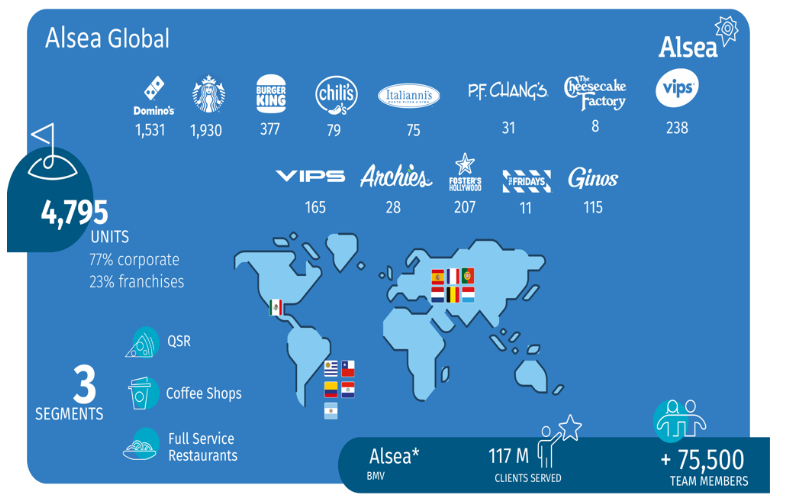
\includegraphics[width=0.7\textwidth]{img/presencia_internacional.png}
  \caption{Mapa de presencia internacional de AESLA (Food Service Project). Fuente: elaboración propia a partir de~\cite{AESLACorporate}.}
  \label{fig:presencia-internacional}
\end{figure}

La magnitud de esta operación internacional hace que AESLA maneje diariamente un volumen muy elevado de información relativa a ventas, operaciones, proyectos de innovación, indicadores de desempeño y actividades internas. En este contexto, disponer de datos fiables, centralizados y fácilmente accesibles resulta fundamental para evaluar el rendimiento de las franquicias, identificar posibles desviaciones y tomar decisiones estratégicas fundamentadas. Sin herramientas de análisis adecuadas, la gestión de este conocimiento se vuelve compleja y poco eficiente.\\

Para dar respuesta a esta necesidad, GBTEC Software AG, compañía alemana especializada en soluciones de gestión de procesos de negocio (\acrfull{bpm}), arquitectura empresarial (\acrfull{eam}) y gobierno, riesgo y cumplimiento (\acrfull{grc}), ofrece la \textit{BIC Platform}, un ecosistema de software que permite modelar, ejecutar y analizar procesos empresariales~\cite{GBTECCorporate,BICPlatformDocs}. Dentro de este marco, se desarrolló para AESLA un módulo específico denominado \textit{Report Service}, cuya finalidad es transformar los datos de la plataforma de Process Execution en informes ejecutivos descargables en formato Excel.\\

La \textit{BIC Platform} se despliega habitualmente en modalidad cloud (BIC Cloud) y está compuesta por varios módulos que cubren el ciclo de vida de los procesos: \textit{Process Design} para modelar procesos mediante diagramas BPMN, y \textit{Process Execution} para ejecutar y automatizar esos procesos, gestionando instancias, tareas y persistencia de variables~\cite{BICPlatformDocs,BPMNStandard}. El \textit{Report Service} extrae información de \textit{Process Execution} (combinada con consultas a \gls{elasticsearch}) para componer informes Excel con \acrshort{kpi}, \gls{retroplanning}, \gls{heatmap} y otras métricas solicitadas por AESLA.\\

\begin{figure}[H]
  \centering
  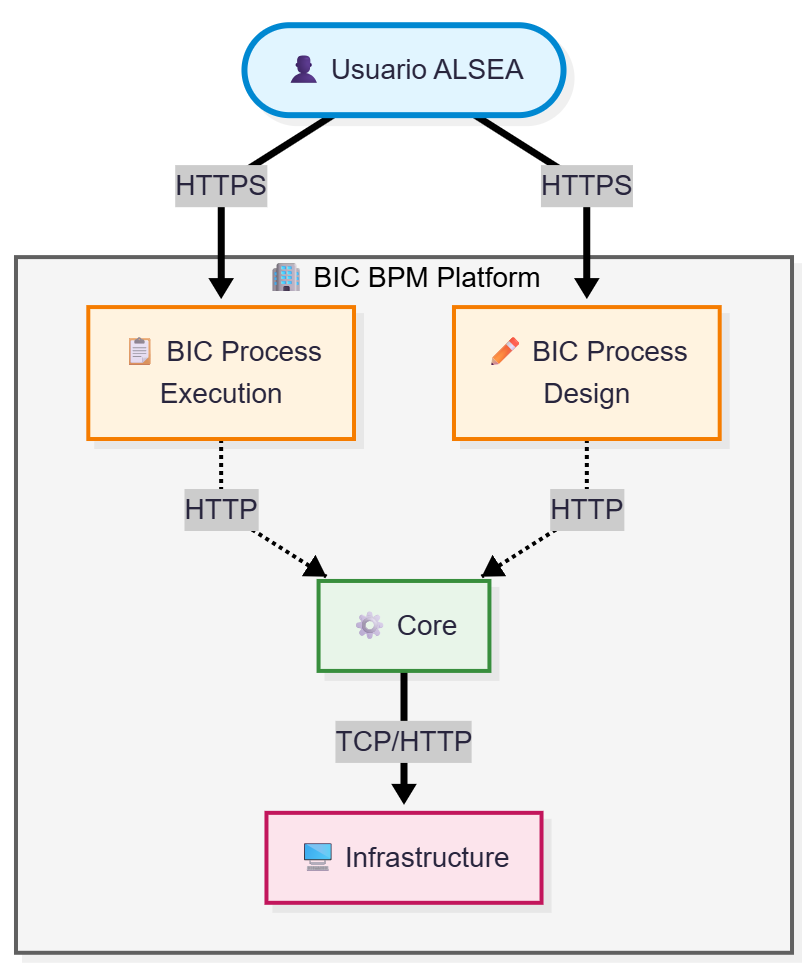
\includegraphics[width=0.85\textwidth]{img/bic_bpm_platform.png}
  \caption{Contexto de la plataforma BIC BPM mostrando la arquitectura de sistemas y sus interacciones. Fuente: elaboración propia a partir de~\cite{BICPlatformDocs}.}
  \label{fig:bic-platform-context}
\end{figure}

La figura~\ref{fig:bic-platform-context} ilustra la arquitectura completa de la plataforma BIC BPM, mostrando cómo el usuario interactúa mediante \acrshort{https} con los módulos \textit{BIC Process Design} y \textit{BIC Process Execution}, que a su vez se comunican con el núcleo (\textit{Core}) y la capa de infraestructura (\textit{Infrastructure}). Esta arquitectura de sistemas distribuidos proporciona la base sobre la que se integra el Report Service desarrollado en este proyecto.\\

Para facilitar la comprensión del papel de \textit{BIC Process Design} dentro de la plataforma, la figura~\ref{fig:bpmn-process-design} muestra un ejemplo sencillo de un proceso de negocio modelado mediante BPMN. Este tipo de diagramas permite representar gráficamente el flujo de un proceso mediante eventos, actividades y decisiones, proporcionando una visión estructurada de las distintas etapas que lo componen.\\ \begin{figure}[H] \centering 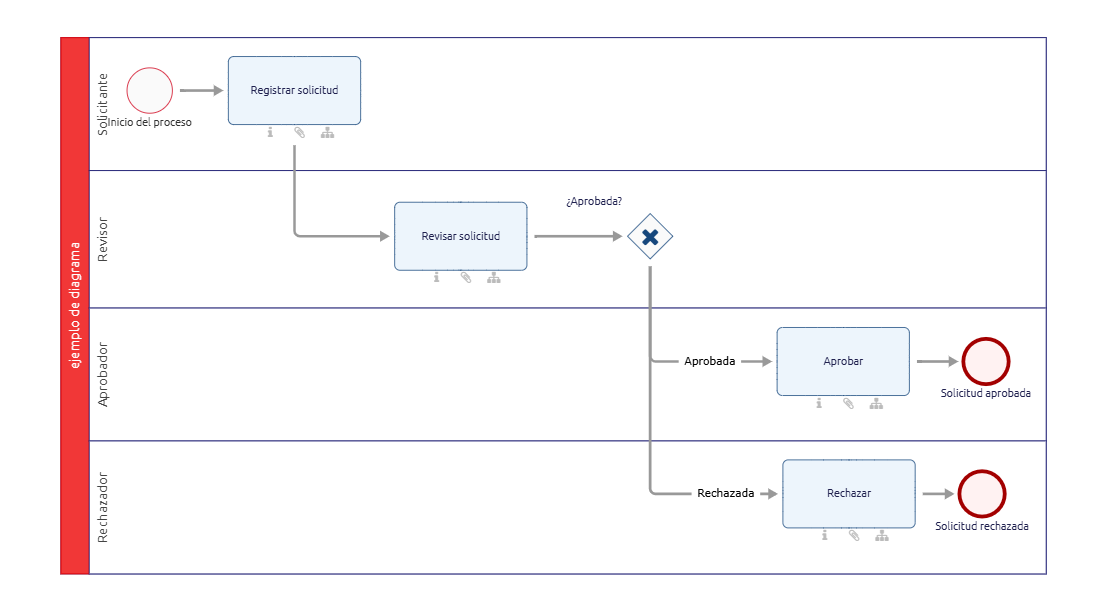
\includegraphics[width=0.9\textwidth]{img/bpmn_process_design.png} \caption{Ejemplo de un proceso BPMN sencillo modelado en BIC Process Design. Fuente: elaboración propia a partir de~\cite{BPMNStandard}.} \label{fig:bpmn-process-design} \end{figure} Los modelos definidos en \textit{Process Design} sirven como representación de los procesos de negocio de la organización. Cuando estos procesos se trasladan al ámbito de ejecución, \textit{Process Execution} permite gestionar sus instancias, tareas y variables asociadas. Parte de esta información constituye posteriormente la fuente de datos utilizada por el \textit{Report Service} para elaborar los informes solicitados por AESLA.\\

El Report Service original ofrecía una solución sencilla y funcional: la interfaz permitía seleccionar el tipo de informe (KPI o Producto), la categoría (Innovación o Alternativa), una o varias franquicias y un rango de fechas. Con esta información, el backend recuperaba los datos correspondientes, generaba un libro de Excel con múltiples hojas y lo devolvía al usuario para su descarga local.\\

Cada combinación produce un libro Excel con múltiples hojas que cubren distintos requisitos y métricas personalizadas solicitadas por el cliente. A continuación se muestran dos ejemplos representativos que ilustran la estructura y contenido de estos informes:

\begin{figure}[H]
  \centering
  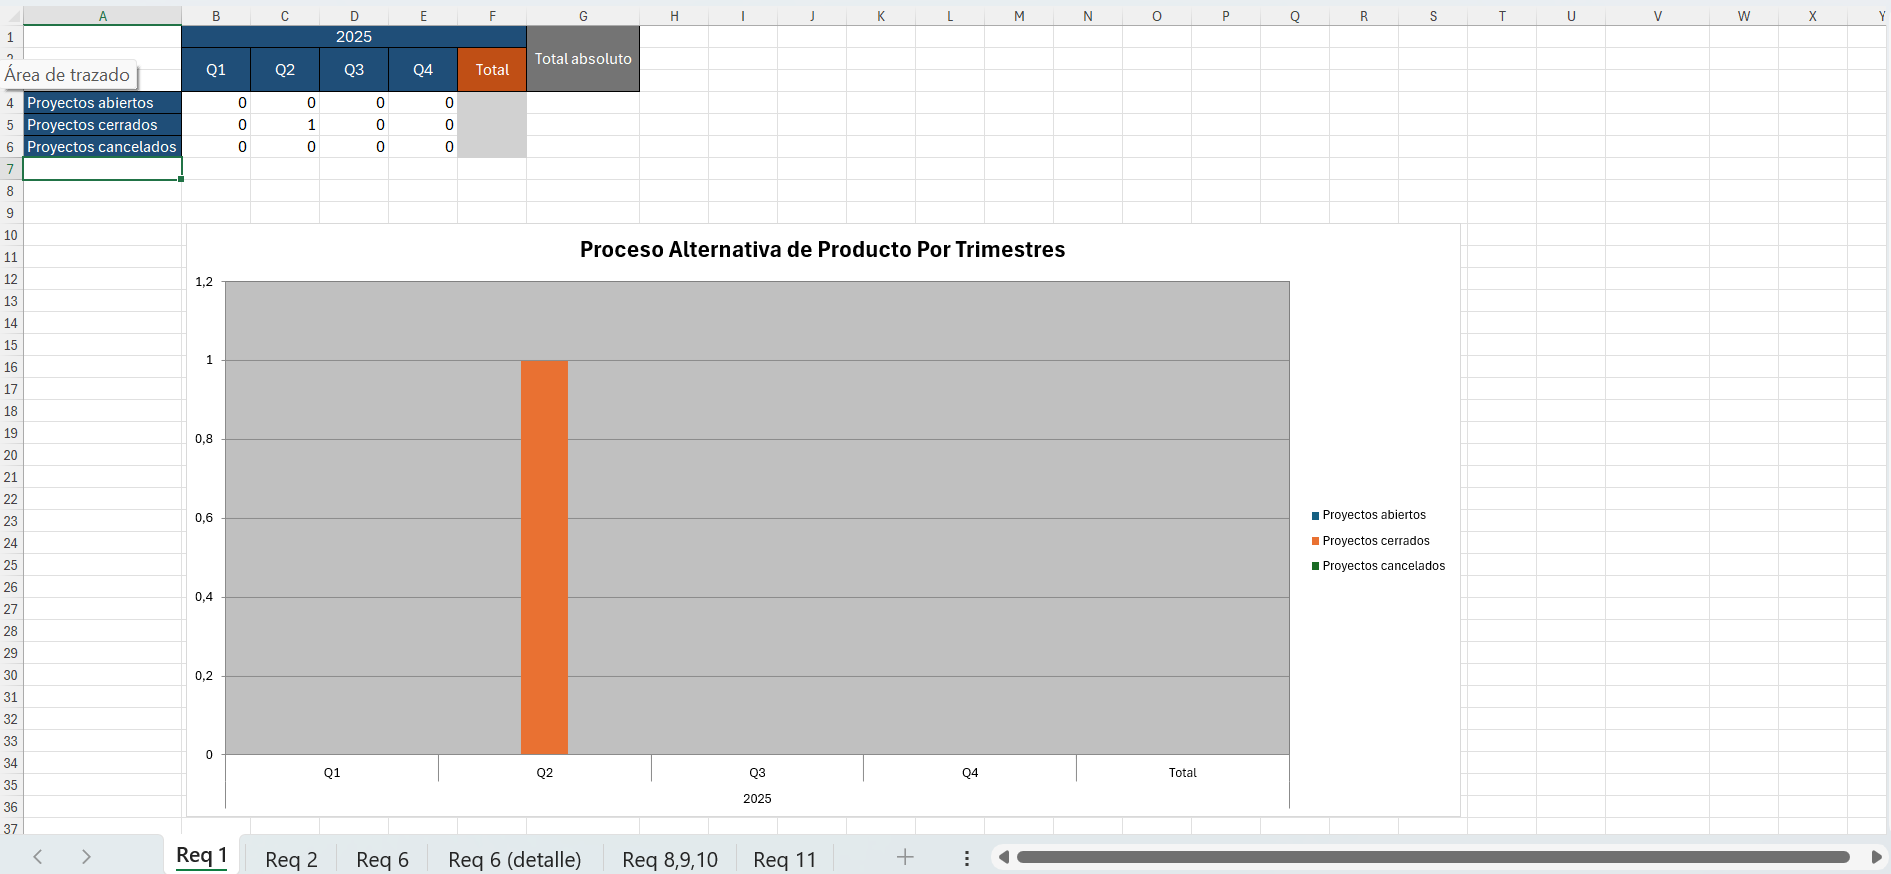
\includegraphics[width=\textwidth]{img/kpi_alternative_todas.png}
  \caption{Informe de tipo KPI con categoría de proceso Alternativa (todas las franquicias, sin rango de fechas).}
  \label{fig:kpi-alternative}
\end{figure}

La anterior figura muestra la hoja del Requisito 1, que presenta un \gls{histograma} con los procesos de alternativa de producto por trimestres, diferenciando proyectos abiertos, cerrados y cancelados, además de los totales y el total absoluto en 2025. En la parte inferior se observan las pestañas de otras hojas del libro, correspondientes a requisitos adicionales personalizados solicitados por el cliente.

\begin{figure}[H]
  \centering
  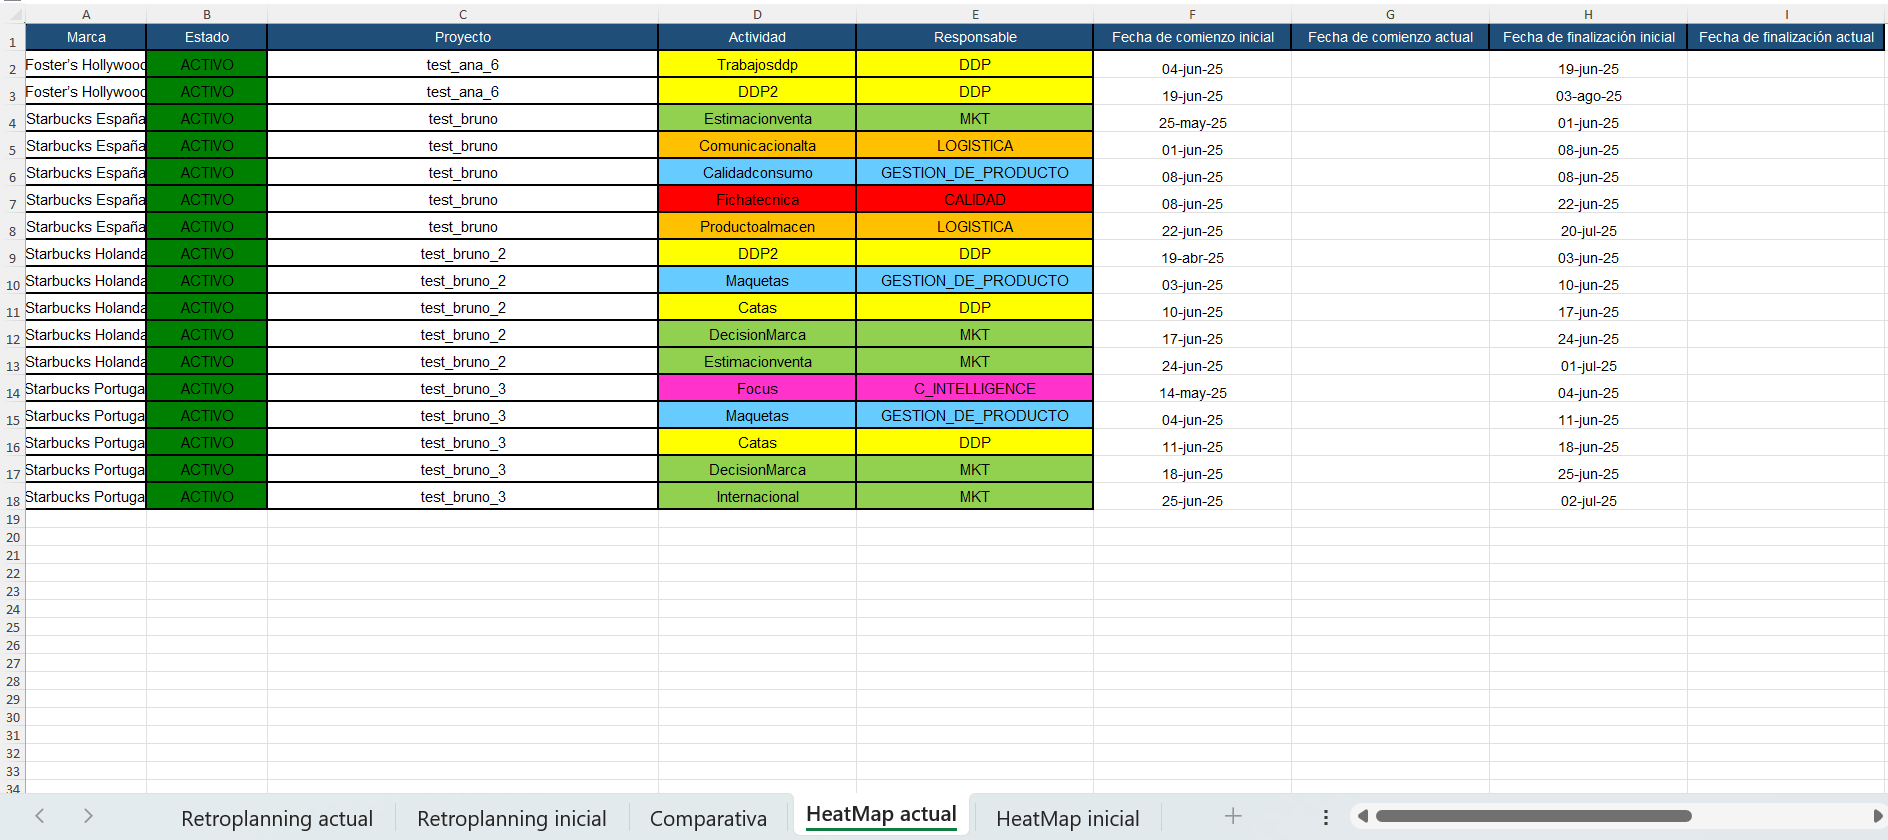
\includegraphics[width=\textwidth]{img/product_innovation_todas.png}
  \caption{Informe de tipo Producto con categoría de proceso Innovación (todas las franquicias, sin rango de fechas).}
  \label{fig:product-innovation}
\end{figure}

La anterior figura muestra la hoja del heatmap actual, que representa para cada marca el estado de sus proyectos junto con las actividades, responsables que las llevan a cabo y fechas previstas. En la parte inferior se pueden observar las pestañas de otras hojas del libro, incluyendo los retroplannings y una hoja de comparativa, que forman parte del conjunto de métricas y análisis solicitados por AESLA.

Estos ejemplos muestran la riqueza informativa y el nivel de personalización de los informes generados por el Report Service, diseñados para cubrir las necesidades analíticas específicas de AESLA en la gestión de sus procesos de innovación y alternativa de producto.\\

Sin embargo, con el paso del tiempo surgieron limitaciones notables. El sistema carecía de un almacenamiento histórico de informes, lo que obligaba a los usuarios a regenerarlos cada vez que deseaban acceder a información pasada. Además, se detectaron problemas de duplicación de código en el backend, ausencia de procesamiento asíncrono (lo que generaba bloqueos en la interfaz durante la creación de los informes) y una experiencia de usuario que no reflejaba plenamente las necesidades de la organización. Estas carencias constituyeron la motivación principal para emprender un proceso de mejora y modernización del Report Service.

\section{Objetivos}

El presente Trabajo de Fin de Grado documenta, analiza y evalúa las mejoras introducidas en el Report Service de AESLA durante mis prácticas en GBTEC. En concreto, se plantearon los siguientes objetivos:

\begin{itemize}
    \item Ampliar la funcionalidad del servicio con almacenamiento histórico en base de datos.
    \item Incrementar la mantenibilidad y calidad del código, reduciendo duplicaciones y aumentando la cobertura de pruebas.
    \item Optimizar la experiencia de usuario en la interfaz de generación de informes y acceso al historial.
    \item Introducir procesamiento asíncrono con \gls{springbatch}, evitando bloqueos en la interfaz.
    \item Añadir control de duplicidad para evitar regeneraciones innecesarias.
    \item Permitir la redescarga de informes desde el historial.
\end{itemize}

Con ello, se pretende transformar el Report Service en una solución completa que cubra tanto la generación como la gestión del ciclo de vida completo de los informes ejecutivos.

 %%%%%%%%%%%%%%%%%%%%%%%%%%%%%%%%%%%%%%%%
 % Capítulo   2                         %
 %%%%%%%%%%%%%%%%%%%%%%%%%%%%%%%%%%%%%%%%

\chapter{Fundamentos tecnológicos}

\section{Estado del arte}

Para la elaboración del estado del arte se han analizado distintas soluciones disponibles en el mercado relacionadas con la generación de informes empresariales y cuadros de mando, evaluando sus ventajas y limitaciones. El objetivo de este análisis es comprender cómo se abordan actualmente estas necesidades en el sector y en qué medida las herramientas existentes inspiran o contrastan con el desarrollo del módulo Report Service en AESLA.\\

\textbf{Microsoft Power BI}\footnote{\url{https://www.microsoft.com/es-es/power-platform/products/power-bi}} es una de las plataformas líderes en el ámbito de la inteligencia de negocio. Destaca por su capacidad de conexión a múltiples fuentes de datos y por ofrecer cuadros de mando interactivos y actualizados en tiempo real. Su principal fortaleza es la flexibilidad de visualización y la posibilidad de integrar gráficos avanzados sin conocimientos de programación. No obstante, entre sus limitaciones se encuentra la complejidad de configuración inicial y la necesidad de licencias específicas para acceder a todas las funcionalidades.\\

\textbf{Tableau}\footnote{\url{https://www.tableau.com/es-es/why-tableau/what-is-tableau}} constituye otra herramienta ampliamente utilizada. Su punto fuerte es la facilidad con la que permite generar visualizaciones intuitivas y estéticamente atractivas. Además, ofrece opciones de colaboración entre equipos y una buena integración con entornos corporativos. Sin embargo, su curva de aprendizaje puede ser elevada para usuarios sin experiencia previa, y su enfoque está más orientado a cuadros de mando interactivos que a informes exportables en formatos tradicionales como Excel.\\

\textbf{Qlik Sense}\footnote{\url{https://www.qlik.com/es-es/products/qlik-sense}} se centra en la exploración de datos y en la creación de dashboards personalizados. Su motor asociativo facilita el análisis de relaciones entre diferentes conjuntos de datos, permitiendo descubrir patrones de forma ágil. Entre sus limitaciones destaca que, al igual que en el caso de Tableau, no siempre resulta la herramienta más adecuada para informes ejecutivos estandarizados en Excel, que siguen siendo demandados en muchos entornos corporativos.\\

\textbf{JasperReports} es una solución orientada a la generación programática de informes a partir de plantillas y fuentes de datos configurables~\cite{JasperReportsDocs}. Este enfoque se aproxima más al problema tratado en este TFG, aunque requiere desarrollar y mantener la lógica específica de integración y generación para cada dominio de negocio.\\

La comparación se resume en la tabla~\ref{tab:comparativa-estado-arte}. Las valoraciones son cualitativas y se refieren a las características descritas en la documentación oficial de cada solución; no constituyen una prueba de rendimiento entre productos.

\begin{table}[H]
  \centering
  \scriptsize
  \caption{Comparación cualitativa de soluciones relacionadas con el análisis
  y la generación de informes.}
  \label{tab:comparativa-estado-arte}
  \rowcolors{2}{udcgray!08}{white}

  \begin{tabularx}{0.98\textwidth}
    {@{}p{0.15\textwidth}
        p{0.20\textwidth}
        p{0.15\textwidth}
        p{0.22\textwidth}
        X@{}}

    \toprule
    \rowcolor{udcpink!20}

    \textbf{Solución} &
    \textbf{Enfoque principal} &
    \textbf{Exportación a Excel} &
    \textbf{Generación de Excel personalizado} &
    \textbf{Integración con BIC} \\

    \midrule

    Power BI~\cite{PowerBIDocs} &
    Inteligencia de negocio y visualización &
    Sí &
    No constituye su objetivo principal; permite exportar datos de
    visualizaciones &
    No específica \\

    Tableau~\cite{TableauDocs} &
    Análisis y visualización interactiva &
    Sí &
    Principalmente exportación de datos o vistas &
    No específica \\

    Qlik Sense~\cite{QlikDocs} &
    Analítica y exploración asociativa &
    Sí &
    Principalmente exportación de datos de visualizaciones &
    No específica \\

    JasperReports~\cite{JasperReportsDocs} &
    Generación programática de informes &
    Sí &
    Sí, mediante plantillas y lógica de generación &
    Requiere integración específica \\

    Report Service &
    Informes específicos sobre procesos BIC &
    Sí &
    Sí, adaptada a los requisitos de AESLA &
    Integración directa con la plataforma \\

    \bottomrule
  \end{tabularx}

  \rowcolors{2}{}{}
\end{table}

Las soluciones analizadas responden a necesidades diferentes. Power BI,
Tableau y Qlik Sense están orientadas principalmente al análisis visual y a
los cuadros de mando, aunque permiten exportar los datos mostrados a formatos
compatibles con Excel. JasperReports se aproxima más al problema tratado en
este proyecto, al proporcionar un motor programático de generación de
informes basado en plantillas. \\

El Report Service presenta, sin embargo, un ámbito más específico: se integra
directamente con los datos y procesos de la plataforma BIC y genera libros
Excel cuya estructura, hojas, métricas y reglas de negocio responden a los
requisitos concretos de AESLA. Por tanto, no pretende sustituir a una
plataforma generalista de inteligencia de negocio, sino resolver una necesidad
de reporting especializada dentro del ecosistema existente. \\

\section{Tecnologías utilizadas}

El desarrollo del Report Service se apoyó en un conjunto de tecnologías que abarcan tanto el cliente web como el servidor y la base de datos, junto con utilidades complementarias para despliegue, monitorización y calidad.

\subsection{Servidor web}

\begin{itemize}
    \item \textbf{Spring Boot}: framework de desarrollo en Java que permite crear aplicaciones web y microservicios de forma rápida y estructurada. Aporta configuración automática, inyección de dependencias y un ecosistema rico de librerías~\cite{SpringBootDocs}.
    \item \textbf{Spring Batch}: módulo de Spring orientado al procesamiento por lotes. Se utilizó para implementar la generación asíncrona de informes, gestionando \textit{jobs} y \textit{steps} de manera controlada~\cite{SpringBatchDocs}.
    \item \textbf{Hibernate / \acrshort{jpa}}: framework de mapeo objeto-relacional que simplifica el acceso a la base de datos mediante entidades Java, evitando tener que escribir consultas \acrshort{sql} manuales~\cite{HibernateDocs}.
    \item \gls{aspose}: es una librería de generación y manipulación de Excel utilizada para dar formato, estilos y estructura a los informes~\cite{AsposeCellsDocs}.
    \item \textbf{Elasticsearch}: motor de búsqueda utilizado como fuente de datos adicional, especialmente para recuperar información de instancias de procesos con consultas \acrshort{json} flexibles~\cite{ElasticsearchDocs}.
    \item \textbf{Maven}: herramienta de gestión y automatización de proyectos Java, empleada para manejar dependencias, construir el proyecto y ejecutar tareas comunes~\cite{MavenDocs}.
\end{itemize}

\subsection{Cliente web}

\begin{itemize}
    \item \textbf{Angular}: framework de desarrollo basado en TypeScript utilizado para construir la interfaz del usuario. Permite crear componentes modulares, mantener un enrutamiento dinámico y gestionar formularios y servicios de forma escalable~\cite{AngularDocs}.
    \item \textbf{Yarn}: gestor de dependencias para proyectos JavaScript que garantiza instalaciones reproducibles y seguras. Fue la herramienta principal para administrar librerías del frontend y realizar auditorías de seguridad.
    \item \textbf{Node.js}: entorno de ejecución necesario para compilar y ejecutar \gls{angular} en local, así como para el servidor de desarrollo.
    \item \textbf{TypeScript}: lenguaje de programación que extiende JavaScript con tipado estático y características avanzadas, facilitando el desarrollo de aplicaciones robustas y mantenibles.
\end{itemize}

\subsection{Base de datos}

\begin{itemize} 
    \item \textbf{PostgreSQL}: sistema de gestión de bases de datos relacional, robusto y de código abierto, empleado para almacenar los informes generados y sus metadatos~\cite{PostgreSQLDocs}.
    \item \textbf{Flyway}: herramienta de migraciones que asegura el versionado y la coherencia del esquema de base de datos en todos los entornos (desarrollo, pruebas y producción). Se utilizó para crear y mantener el esquema \texttt{aesla\_reports} y su tabla principal \texttt{report}~\cite{FlywayDocs}.
    \item \textbf{Testcontainers}: framework de testing que permite levantar contenedores efímeros de \gls{postgresql} durante la ejecución de pruebas, garantizando un entorno controlado y reproducible~\cite{TestcontainersDocs}.
\end{itemize}

\subsection{Infraestructura y Despliegue}

\begin{itemize}
    \item \textbf{Docker}: plataforma de contenedores utilizada para empaquetar tanto el backend como el frontend y garantizar despliegues reproducibles en diferentes entornos~\cite{DockerDocs}.
    \item \textbf{Git}: sistema de control de versiones empleado en combinación con ramas de funcionalidad y \textit{Pull Requests}, asegurando trazabilidad y revisiones de código antes de su integración.
\end{itemize}

\subsection{Herramientas de apoyo}

\begin{itemize}
  \item \textbf{Gestión de trabajo}: \gls{jira} se utilizó junto con un tablero \gls{kanban} para organizar elementos de tipo \textit{Epic}, historias de usuario y subtareas, así como para gestionar prioridades y realizar el seguimiento visual del progreso de cada ticket~\cite{JiraDocs}.
  \item \textbf{Control de versiones y hosting}: Git para control de versiones y GitHub como repositorio remoto centralizado donde se alojaba el código fuente del proyecto, facilitando la colaboración mediante Pull Requests y revisiones de código.
  \item \textbf{Flujo de trabajo Git}: \gls{gitflow}~\cite{Gitflow} se adoptó como convención de ramas (feature/fix/hotfix) para mantener estabilidad en las ramas de producción y organizar el desarrollo de forma estructurada.
  \item \textbf{Integración continua / \acrshort{ci} \& CD}: \gls{githubactions} se configuró con acciones personalizadas para automatizar el build del proyecto, ejecutar pruebas unitarias e integradas, y realizar despliegues~\cite{GitHubActionsDocs}. Los pipelines se integraron con SonarQube (SonarCloud) para validar métricas de calidad de código (\gls{coverage}, \gls{duplicacion}, \gls{codesmells}) antes de aceptar cada \acrshort{pr}~\cite{SonarQubeDocs}.
  \item \textbf{Registro y gestión de artefactos}: \gls{quay} se empleó como registry principal para almacenar y versionar las imágenes Docker de los entornos Ansible de prueba, mientras que \gls{jfrog} sirvió como repositorio de artefactos binarios y dependencias Maven/NPM, facilitando la distribución controlada de versiones.
  \item \textbf{Orquestación de despliegue y automatización}: \gls{ansible} (gestionado mediante \acrshort{awx}) permitió levantar entornos de prueba y automatizar despliegues en \acrshort{qa}.
  \item \textbf{Entornos de desarrollo}: IntelliJ IDEA para backend (Java/Spring) y Visual Studio Code para frontend (Angular/TypeScript).
  \item \textbf{Pruebas y depuración}: \gls{postman} para pruebas de \acrshort{api} y Google Chrome para pruebas manuales en entorno local.
  \item \textbf{Calidad de código}: \gls{sonarcloud} / SonarQube se integró en los pipelines de \acrshort{ci} para realizar análisis estático de código (\acrshort{html}, \acrshort{css}, TypeScript, Java), medir cobertura de pruebas, detectar duplicaciones y controlar la deuda técnica, garantizando que cada cambio cumpliera con los umbrales de calidad definidos por la empresa.
\end{itemize}

 %%%%%%%%%%%%%%%%%%%%%%%%%%%%%%%%%%%%%%%%
 % Capítulo   3                         %
 %%%%%%%%%%%%%%%%%%%%%%%%%%%%%%%%%%%%%%%%

\chapter{Metodología y planificación}

\section{Metodología de desarrollo}

El proyecto se llevó a cabo siguiendo una metodología ágil~\cite{AgileManifesto} basada en iteraciones cortas y gestión Kanban~\cite{AndersonKanban} en \gls{jira}. Este enfoque resultó adecuado por la naturaleza incremental de las mejoras del Report Service, la necesidad de integrar cambios en backend y frontend con validación continua, y la conveniencia de priorizar incidencias, tareas técnicas y funcionalidades nuevas. Este tablero Kanban se configuró con el objetivo de permitir visualizar el flujo de trabajo completo, con estados definidos (\texttt{To Do} → \texttt{Task Breakdown} → \texttt{In Progress} → \texttt{Ready for QA/PR} → \texttt{QA/PR OK} → \texttt{Done}) para cada tarea, facilitando el seguimiento de prioridades y la identificación de bloqueos.\\

Las características principales del enfoque fueron:

\begin{itemize}
  \item \textbf{Iterativo e incremental}: cada conjunto de cambios (feature/refactor/fix/chore) se gestionó como un elemento de trabajo en el tablero, produciendo un incremento funcional verificable (código, tests y PR).
  \item \textbf{Retroalimentación continua}: reuniones diarias con el equipo para sincronizar prioridades, desbloquear tareas y validar entregables; revisión de PRs con comentarios técnicos.
  \item \textbf{Flexibilidad}: replanificación rápida en función de prioridades del \acrshort{epic} y de incidencias no previstas inicialmente que surgieron durante el desarrollo (p.\,ej., unificación de estructuras de peticiones entre tipos de informe, compatibilidad de parámetros opcionales como fechas nulas, detección de duplicidades), las cuales se integraron de manera ágil en las tareas correspondientes.
\end{itemize}

\subsection{Adaptación al proyecto}

La incorporación al proyecto siguió una fase breve de formación, alineada con las tecnologías clave:

\begin{itemize}
  \item \textbf{Formación inicial}: cursos introductorios de Spring Batch, \gls{docker}, patrones de diseño en Java y Angular (priorizando primero el backend), proporcionados mediante la suscripción de Udemy contratada por la empresa.
  \item \textbf{Aterrizaje en Jira}: asignación al \acrshort{epic} \textit{Improvements for AESLA Project in 2025 Q3 \& Q4}, que agrupaba los work items relacionados con la evolución del Report Service. La mayoría se clasificaron como \textit{Task}, aunque también se gestionaron incidencias de tipo \textit{Bug} y una historia de usuario de mayor alcance para introducir la generación asíncrona.
  \item \textbf{Flujo de trabajo}:
    \begin{itemize}
      \item Rama por tarea (feature/fix branch) en Git.
      \item Commits atómicos y descriptivos.
      \item Pull Request hacia \texttt{development}, con code review y checks automáticos de SonarCloud y build de pull/push.
      \item Cierre de la tarea al completar \acrshort{pr} y \acrshort{qa}.
      \item Uso de una misma \textit{fix version} del Report Service para agrupar los cambios que debían publicarse conjuntamente.
    \end{itemize}
\end{itemize}

El orden de adaptación técnica fue: backend → datos → frontend, permitiendo una integración progresiva. Para cada work item se creó una rama independiente en Git, identificada con el número de la tarea, donde se realizaron los commits correspondientes. Una vez finalizado el desarrollo y superada la revisión de código y la validación de QA, se aprobaba el Pull Request y se integraban los cambios en la rama \texttt{development} del Report Service.

\section{Planificación y seguimiento}

El proyecto se desarrolló durante los meses de julio, agosto y septiembre. La dedicación al trabajo fue de 7 horas diarias durante julio y agosto, y de 6 horas diarias durante septiembre, al tener que compaginar las prácticas con el inicio del curso universitario.

La planificación del proyecto se estructuró en fases de trabajo, en lugar de \textit{sprints} formales, de acuerdo con la metodología ágil basada en Kanban utilizada por el equipo. Esta forma de organización permitió adaptar el ritmo de trabajo y la prioridad de las tareas a las necesidades reales del proyecto, manteniendo un seguimiento continuo del estado de cada \textit{work item}.

Con el objetivo de reflejar tanto la previsión inicial como la evolución efectiva del proyecto, se presentan dos diagramas de Gantt: uno correspondiente a la \textbf{planificación inicial} y otro al \textbf{seguimiento real}. La comparación entre ambos permite identificar de forma visual las fases que se prolongaron más de lo previsto inicialmente.

\subsection{Planificación inicial}

La planificación inicial se definió de forma orientativa al comienzo del proyecto. En ella se preveía una primera fase breve de incorporación y formación, seguida por tareas de refactorización y limpieza del código. Posteriormente se abordaría la unificación de la gestión de informes y la evolución del backend como núcleo principal del trabajo. Finalmente, la integración del frontend se reservaría para septiembre, dejando la última semana para las tareas de cierre, liberación de versión y documentación.

\begin{figure}[H]
\centering
\resizebox{\textwidth}{!}{
\begin{ganttchart}[
    hgrid,
    vgrid,
    x unit=0.85cm,
    y unit chart=0.7cm,
    bar height=0.5,
    title height=1,
    title/.style={fill=gray!15},
    bar/.style={fill=blue!35},
    bar label font=\small,
    title label font=\small\bfseries
]{1}{12}

\gantttitle{Julio}{4}
\gantttitle{Agosto}{4}
\gantttitle{Septiembre}{4} \\

\gantttitle{S1}{1}
\gantttitle{S2}{1}
\gantttitle{S3}{1}
\gantttitle{S4}{1}
\gantttitle{S1}{1}
\gantttitle{S2}{1}
\gantttitle{S3}{1}
\gantttitle{S4}{1}
\gantttitle{S1}{1}
\gantttitle{S2}{1}
\gantttitle{S3}{1}
\gantttitle{S4}{1} \\

\ganttbar{Onboarding y formación}{1}{1} \\
\ganttbar{Limpieza y refactors}{1}{3} \\
\ganttbar{Unificación de informes}{3}{4} \\
\ganttbar{Evolución backend}{4}{7} \\
\ganttbar{Pruebas y validación}{5}{8} \\
\ganttbar{Formación Angular e integración frontend}{9}{11} \\
\ganttbar{Cierre, release y documentación}{12}{12}

\end{ganttchart}
}
\caption{Diagrama de Gantt de la planificación inicial del proyecto.}
\label{fig:gantt-plan-inicial}
\end{figure}

Como puede observarse, la planificación inicial planteaba una secuencia relativamente ordenada: una primera fase de adaptación durante la primera semana de julio, una etapa de refactorización durante el resto del mes, la transición hacia la unificación del servicio entre finales de julio y comienzos de agosto, el desarrollo del backend como fase central del proyecto, y finalmente la integración del frontend y el cierre durante septiembre.

\subsection{Seguimiento real}

Durante la ejecución del proyecto, la planificación inicial tuvo que adaptarse a las necesidades que fueron surgiendo, en coherencia con la metodología ágil empleada. Algunas tareas previstas resultaron más complejas de lo estimado inicialmente, especialmente aquellas relacionadas con la unificación de la gestión de informes y la evolución del backend.

La unificación de la gestión de informes se prolongó más de lo previsto porque implicó homogeneizar controladores, endpoints y DTOs, así como normalizar el tratamiento de parámetros opcionales y reorganizar la estructura interna de paquetes. Del mismo modo, la evolución del backend también requirió más tiempo, al incorporar persistencia de informes, endpoints de consulta y descarga, generación asíncrona con Spring Batch, control de duplicidad, registro de métricas y ajustes relacionados con la inicialización de Flyway y de las tablas asociadas a Spring Batch.

Además, las pruebas y validaciones no se limitaron a una fase puntual, sino que se mantuvieron a lo largo de buena parte del desarrollo, en forma de pruebas unitarias, integradas, revisión de \textit{Pull Requests} y validación en QA. Como consecuencia, varias actividades se solaparon parcialmente sin alterar la fecha final de cierre del proyecto.

\begin{figure}[H]
\centering
\resizebox{\textwidth}{!}{
\begin{ganttchart}[
    hgrid,
    vgrid,
    x unit=0.85cm,
    y unit chart=0.7cm,
    bar height=0.5,
    title height=1,
    title/.style={fill=gray!15},
    bar/.style={fill=green!35},
    bar label font=\small,
    title label font=\small\bfseries
]{1}{12}

\gantttitle{Julio}{4}
\gantttitle{Agosto}{4}
\gantttitle{Septiembre}{4} \\

\gantttitle{S1}{1}
\gantttitle{S2}{1}
\gantttitle{S3}{1}
\gantttitle{S4}{1}
\gantttitle{S1}{1}
\gantttitle{S2}{1}
\gantttitle{S3}{1}
\gantttitle{S4}{1}
\gantttitle{S1}{1}
\gantttitle{S2}{1}
\gantttitle{S3}{1}
\gantttitle{S4}{1} \\

\ganttbar{Onboarding y formación}{1}{1} \\
\ganttbar{Limpieza y refactors}{1}{4} \\
\ganttbar{Unificación de informes}{3}{6} \\
\ganttbar{Evolución backend}{4}{9} \\
\ganttbar{Pruebas y validación}{2}{11} \\
\ganttbar{Formación Angular e integración frontend}{9}{11} \\
\ganttbar{Cierre, release y documentación}{12}{12}

\end{ganttchart}
}
\caption{Diagrama de Gantt correspondiente al seguimiento real del proyecto.}
\label{fig:gantt-seguimiento-real}
\end{figure}

La comparación entre ambos diagramas muestra que las principales desviaciones se produjeron en la fase de unificación de la gestión de informes y en la fase de evolución backend, ambas con una duración superior a la prevista inicialmente. Asimismo, las pruebas y validación adquirieron un carácter transversal, acompañando al desarrollo durante gran parte del proyecto. No obstante, estas desviaciones no afectaron al cumplimiento de los objetivos ni al cierre del proyecto dentro del periodo inicialmente establecido.

 %%%%%%%%%%%%%%%%%%%%%%%%%%%%%%%%%%%%%%%%
 % Capítulo   4                         %
 %%%%%%%%%%%%%%%%%%%%%%%%%%%%%%%%%%%%%%%%

\chapter{Análisis}

\section{Requisitos}

\subsection{Actores y Sistemas involucrados}
En el sistema intervienen distintos actores y componentes que participan en la generación, almacenamiento y consulta de los informes ejecutivos:

\begin{itemize}
    \item \textbf{Usuario AESLA}: empleado o analista encargado de generar y consultar los informes a través de la interfaz web. Puede lanzar nuevas generaciones, visualizar el historial y volver a descargar informes anteriores.
    \item \textbf{Aplicación web}: cliente desarrollado en Angular que permite la interacción del usuario con el sistema. Presenta formularios, mensajes de estado y botones de acción, y consulta periódicamente el estado de la generación mediante el endpoint \texttt{/api/reports/latest}.
    \item \textbf{Servicio de reportes}: aplicación de servidor desarrollada con Spring Boot. Gestiona la lógica de negocio, coordina la generación asíncrona de informes, controla la duplicidad y persiste los resultados.
    \item \textbf{Origen de datos de procesos}: base de datos de ejecución de procesos de BIC (BIC Process Execution) y fuentes adicionales en \textit{Elasticsearch}, de donde se obtienen las variables necesarias para la composición de los informes.
    \item \textbf{Base de datos de informes}: sistema PostgreSQL donde se almacenan los informes generados, junto con sus metadatos (categoría, tipo, fechas, franquicias, tamaño, etc.).
\end{itemize}

\subsection{Requisitos funcionales}
Los requisitos funcionales definen el comportamiento observable del sistema y las acciones que el usuario puede realizar:

\begin{enumerate}
    \item \textbf{RF-01 - Generación de informes}:
    \begin{itemize}
        \item El sistema debe permitir la generación de informes en formato Excel, ofreciendo la posibilidad de seleccionar los siguientes parámetros: \textit{tipo} (KPI o Producto), \textit{categoría} (Innovación o Alternativa), \textit{franquicia(s)} (una, varias o todas) y \textit{rango de fechas} (opcional), que por defecto abarcará desde el inicio de la disponibilidad de datos.
        \item La generación se debe realizar de forma asíncrona, sin bloquear la interfaz.
        \item La aplicación debe mostrar mensajes informativos durante la generación y su seguimiento mediante \textit{polling}: \textit{“Comprobando solicitud”}, \textit{“Generando informe”}, \textit{“Descarga iniciada”}, \textit{“Error de red”} o \textit{“Informe reciente disponible en la pestaña Historial”}.
    \end{itemize}

    \item \textbf{RF-02 - Control de duplicidad}:
    \begin{itemize}
        \item Antes de generar un nuevo informe, el sistema debe comprobar si existe un informe idéntico generado recientemente (p. ej., en los últimos 5 minutos).
        \item En caso afirmativo, se debe bloquear la nueva generación y notificar al usuario que el informe ya está disponible en el historial.
        \item Para realizar esta comprobación, se genera una firma única basada en los parámetros de entrada.
    \end{itemize}

    \item \textbf{RF-03 - Descarga y redescarga de informes}:
    \begin{itemize}
        \item Al finalizar una generación válida, el informe debe quedar disponible para su descarga desde la interfaz del usuario.
        \item El informe debe almacenarse en la base de datos para su consulta futura.
        \item El usuario podrá volver a descargar cualquier informe desde la pestaña \textit{Historial}.
    \end{itemize}

    \item \textbf{RF-04 - Historial de informes}:
    \begin{itemize}
        \item El sistema debe disponer de una página de \textit{Historial} que muestre todos los informes generados, junto con sus metadatos: fecha de creación, categoría de proceso, tipo de informe, franquicias a las que hace referencia (marcas) y rango de fechas.
        \item El historial debe estar ordenado de forma descendente (más recientes primero).
        \item Debe implementarse paginación mediante botones \textit{“5 anteriores”} y \textit{“5 siguientes”}.
    \end{itemize}
\end{enumerate}

\subsection{Requisitos no funcionales}
Los requisitos no funcionales garantizan la calidad y las propiedades del sistema:

\begin{itemize}
    \item \textbf{RNF-01 - Usabilidad}: interfaz simple e intuitiva, con botones y mensajes claros que guíen al usuario en todo momento.
    \item \textbf{RNF-02 - Rendimiento}: la ejecución de informes no debe bloquear la aplicación; la respuesta del historial debe ser inmediata.
    \item \textbf{RNF-03 - Confiabilidad}: almacenamiento persistente en base de datos; control de duplicidad para evitar sobrecarga.
    \item \textbf{RNF-04 - Mantenibilidad}: estructura modular en capas (controladores, servicios, utilidades) y cobertura de pruebas unitarias e integradas.
    \item \textbf{RNF-05 - Escalabilidad}: la arquitectura debe permitir la ejecución asíncrona de trabajos y facilitar una futura ampliación de la capacidad de procesamiento sin requerir cambios sustanciales en el flujo funcional.
    \item \textbf{RNF-06 - Seguridad}: integración con los mecanismos de autenticación y autorización proporcionados por la plataforma BIC, junto con la protección del contenido de los informes.
    \item \textbf{RNF-07 - Observabilidad}: registro de métricas, logs estructurados y seguimiento de procesos.
    \item \textbf{RNF-08 - Compatibilidad}: funcionamiento correcto en navegadores modernos y exportación a formatos Excel estándar.
\end{itemize}

\subsection{Historias de usuario}
A continuación se detallan las principales historias de usuario definidas para el proyecto:

\begin{itemize}
    \item \textbf{HU01 – Generar informe}: 
    Como usuario, quiero seleccionar los parámetros de tipo, categoría, franquicias y rango de fechas para generar un informe Excel personalizado.
    
    \item \textbf{HU02 – Visualizar estados de generación}: 
    Como usuario, quiero recibir notificaciones sobre el estado del informe (comprobando, generando, completado, error, duplicado) para conocer el progreso.

    \item \textbf{HU03 – Control de duplicidad}: 
    Como usuario, quiero que el sistema detecte y bloquee la generación de informes idénticos para evitar duplicidades innecesarias.

    \item \textbf{HU04 – Descarga del informe}: 
      Como usuario, quiero descargar el informe una vez que la generación haya finalizado.

    \item \textbf{HU05 – Historial de informes}: 
    Como usuario, quiero poder consultar un listado con todos los informes generados, ver su información.

    \item \textbf{HU06 – Redescarga}: 
    Como usuario, quiero volver a descargar un informe anterior sin tener que generarlo de nuevo.
\end{itemize}

\begin{figure}[H]
  \centering

  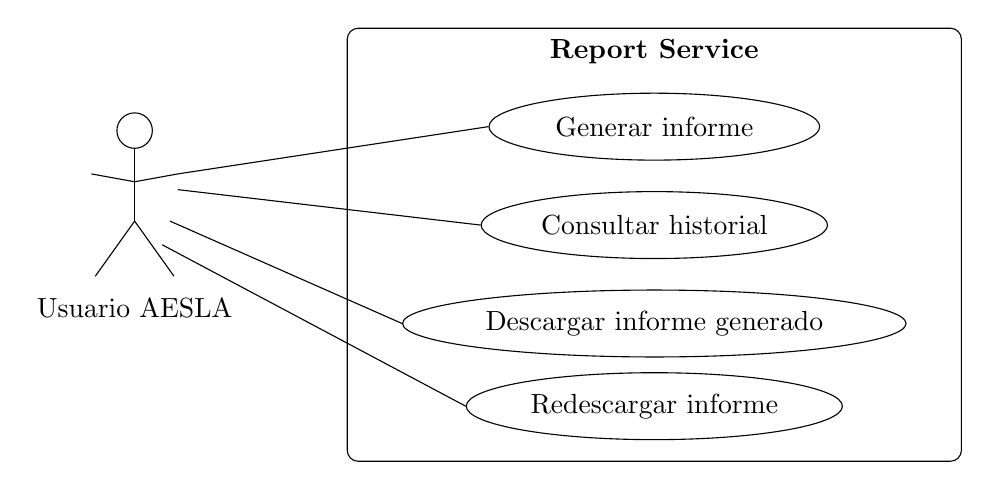
\begin{tikzpicture}[
    usecase/.style={
      draw,
      ellipse,
      align=center,
      minimum width=4.2cm,
      minimum height=0.85cm
    }
  ]

    % Actor
    \node[draw, circle, minimum size=0.45cm, inner sep=0pt] (head) at (0,1.2) {};
    \draw (0,0.97) -- (0,0.05);
    \draw (-0.55,0.65) -- (0,0.55) -- (0.55,0.65);
    \draw (0,0.05) -- (-0.5,-0.65);
    \draw (0,0.05) -- (0.5,-0.65);
    \node at (0,-1.05) {Usuario AESLA};

    % Límite del sistema
    \draw[rounded corners]
      (2.7,2.5) rectangle (10.5,-3.0);

    \node[font=\bfseries] at (6.6,2.2)
      {Report Service};

    % Casos de uso
    \node[usecase] (generate) at (6.6,1.25)
      {Generar informe};

    \node[usecase] (history) at (6.6,0)
      {Consultar historial};

    \node[usecase] (download) at (6.6,-1.25)
      {Descargar informe generado};

    \node[usecase] (redownload) at (6.6,-2.3)
      {Redescargar informe};

    % Asociaciones
    \draw (0.55,0.65) -- (generate.west);
    \draw (0.55,0.45) -- (history.west);
    \draw (0.45,0.05) -- (download.west);
    \draw (0.35,-0.25) -- (redownload.west);

  \end{tikzpicture}

  \caption{Diagrama de casos de uso principales del Report Service. Fuente: elaboración propia.}
  \label{fig:casos-uso}
\end{figure}

La figura~\ref{fig:casos-uso} resume las principales funcionalidades accesibles
para el usuario. El seguimiento del estado mediante \textit{polling}, el control
de duplicidad y la comprobación de disponibilidad de datos forman parte del
comportamiento interno asociado al caso de uso de generación de informes.

\section{Arquitectura del sistema}
La aplicación sigue una arquitectura cliente-servidor basada en servicios web \acrshort{rest} y procesamiento asíncrono. En este capítulo se presenta una visión funcional de los actores y responsabilidades principales; la descripción técnica detallada de paquetes, clases y flujo de ejecución se desarrolla en el capítulo~5.

\subsection{Cliente web}
El cliente web, desarrollado en Angular, gestiona la interacción del usuario y las peticiones al servidor:
\begin{itemize}
    \item Página principal: módulo \textit{Report Generator}, donde se configuran los parámetros y se lanza la generación.
    \item Página secundaria: módulo \textit{Report History}, donde se visualizan y descargan los informes existentes.
    \item Comunicación con el servidor mediante servicios \acrshort{http}, con notificaciones de estado y validaciones de entrada.
\end{itemize}

\subsection{Servidor}
El servidor gestiona la lógica principal:
\begin{itemize}
    \item Controladores REST que reciben solicitudes de generación.
    \item Servicios de coordinación que controlan la duplicidad y comprueban la disponibilidad de datos antes y durante la ejecución del job.
    \item Ejecución asíncrona mediante Spring Batch, con jobs y steps configurables.
    \item Persistencia de resultados y metadatos en PostgreSQL.
    \item Generación de ficheros Excel con Aspose Cells.
\end{itemize}

\subsection{Capa de datos}
\begin{itemize}
    \item Fuentes de información: BIC Process Execution y Elasticsearch, de las que se extraen las variables necesarias.
    \item Almacenamiento: PostgreSQL con migraciones controladas por Flyway.
\end{itemize}

El flujo funcional comienza en el cliente Angular, que envía la solicitud al controlador REST. El servidor valida los parámetros, comprueba posibles duplicidades y, si la solicitud es válida, lanza un job de Spring Batch. El tasklet comprueba la disponibilidad de datos, selecciona el generador KPI o Producto correspondiente, obtiene y transforma los datos, crea el workbook y lo almacena en PostgreSQL. Mientras el job se ejecuta, el frontend consulta periódicamente el endpoint \texttt{/api/reports/latest} con los parámetros de la solicitud. Cuando la respuesta indica que el informe está disponible, el cliente inicia automáticamente la descarga; si no, continúa consultando hasta alcanzar el tiempo máximo configurado.\\

\section{Interfaz de usuario}

La interfaz de usuario original del Report Service presentaba un diseño sencillo y funcional, pero con limitaciones evidentes desde el punto de vista de la experiencia de usuario. Se trataba de una única página web donde el usuario podía configurar los parámetros básicos del informe: tipo (KPI o Producto), categoría (Innovación o Alternativa), selección de franquicias y un rango de fechas opcional.\\

Una vez configurados estos parámetros, el usuario podía solicitar la generación del informe mediante un botón de descarga. En la versión original, el sistema procesaba la solicitud de forma síncrona, bloqueando la interfaz durante todo el proceso de generación, lo que podía resultar en tiempos de espera prolongados sin retroalimentación clara sobre el estado del proceso. Al finalizar, el informe Excel se descargaba directamente al navegador del usuario.\\

El diseño inicial, aunque funcional, presentaba carencias de usabilidad. Las principales limitaciones eran: ausencia de historial, falta de retroalimentación durante la generación, procesamiento síncrono que bloqueaba la interfaz, diseño anticuado y ausencia de control de duplicidad. Estas carencias motivaron el desarrollo de una nueva interfaz modernizada (capítulo 7).\\

\begin{figure}[H]
  \centering
  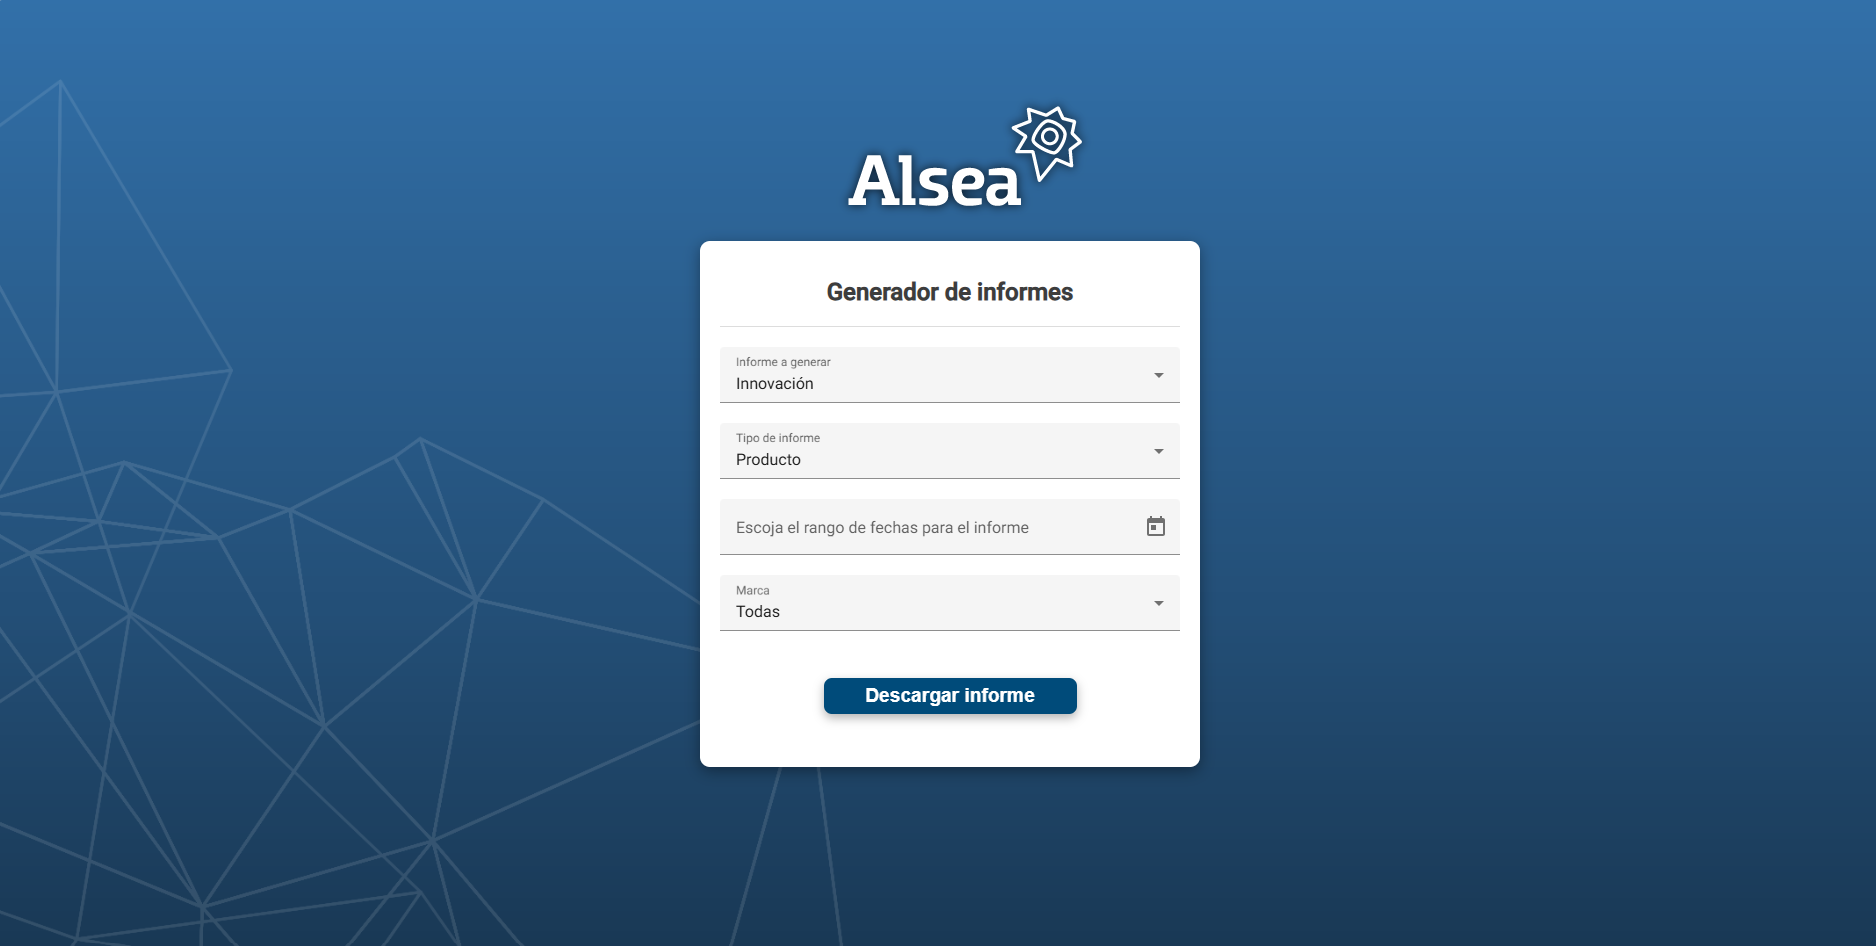
\includegraphics[width=0.9\textwidth]{img/oldui.png}
  \caption{Interfaz original del Report Service antes de su modernización.}
  \label{fig:interfaz-antigua}
\end{figure}


 %%%%%%%%%%%%%%%%%%%%%%%%%%%%%%%%%%%%%%%%
 % Capítulo   5                         %
 %%%%%%%%%%%%%%%%%%%%%%%%%%%%%%%%%%%%%%%%

%%%%%%%%%%%%%%%%%%%%%%%%%%%%%%%%%%%%%%%%%
% Capítulo 5                            %
%%%%%%%%%%%%%%%%%%%%%%%%%%%%%%%%%%%%%%%%%

\chapter{Diseño}

\section{Arquitectura tecnológica del sistema}

En este apartado se describe la estructura final del Report Service
modernizado, justificando las principales decisiones técnicas y explicando
cómo interactúan los diferentes componentes que participan en la generación,
almacenamiento, consulta y descarga de informes.

\subsection{Visión general de la arquitectura}

El Report Service sigue una arquitectura cliente-servidor organizada en tres
capas principales ---presentación, lógica de aplicación y datos---,
complementadas por los componentes de infraestructura necesarios para la
migración de base de datos, contenerización y despliegue. Esta separación
permite distribuir las responsabilidades del sistema y facilita su
mantenimiento y evolución.

\begin{itemize}

  \item \textbf{Capa de presentación}: aplicación web desarrollada en
  Angular 15 que proporciona la interfaz necesaria para configurar la
  generación de informes, consultar su estado, acceder al historial y
  descargar informes previamente generados.

  \item \textbf{Capa de lógica de aplicación}: backend basado en Spring Boot
  3 y Spring Batch encargado de recibir las peticiones, realizar las
  validaciones necesarias, comprobar la duplicidad, coordinar la generación
  asíncrona y gestionar el almacenamiento de los resultados.

  \item \textbf{Capa de datos}: PostgreSQL almacena los informes generados y
  sus metadatos, mientras que Elasticsearch y BIC Process Execution actúan
  como fuentes de información para la construcción de los diferentes tipos
  de informe.

\end{itemize}

La tabla~\ref{tab:componentes-responsabilidades} resume los componentes más
relevantes del sistema y sus responsabilidades.

\begin{table}[H]
  \centering
  \small
  \caption{Componentes principales y responsabilidades del Report Service.}
  \label{tab:componentes-responsabilidades}

  \begin{tabularx}{0.95\textwidth}{@{}p{0.29\textwidth}X@{}}
    \toprule
    \textbf{Componente} &
    \textbf{Responsabilidad principal} \\
    \midrule

    Cliente Angular &
    Recoger los parámetros, validar la entrada, mostrar el estado de la
    solicitud y permitir consultar y descargar informes. \\

    \texttt{ReportBatchController} &
    Exponer los endpoints REST necesarios para iniciar generaciones,
    consultar el estado y el historial y solicitar descargas. \\

    \texttt{ReportLaunchService} &
    Coordinar la comprobación previa de duplicidad y el lanzamiento
    asíncrono del job. \\

    \texttt{ReportDuplicateUtils} &
    Calcular la firma de la solicitud y facilitar la detección de solicitudes
    equivalentes desencadenadas recientemente. \\

    \texttt{GenerateReportTasklet} &
    Coordinar la ejecución del job, comprobar la disponibilidad de datos,
    seleccionar el generador correspondiente y delegar el almacenamiento del
    resultado. \\

    \texttt{ReportDataProbeService} &
    Comprobar si existen datos suficientes para los parámetros solicitados
    antes de ejecutar la generación completa del informe. \\

    \texttt{ReportService} &
    Gestionar la serialización, persistencia y recuperación de los informes
    generados. \\

    \texttt{ReportRepository} &
    Proporcionar mediante JPA el acceso a los informes almacenados en
    PostgreSQL. \\

    \bottomrule
  \end{tabularx}
\end{table}

La figura~\ref{fig:arquitectura-simplificada} muestra de forma resumida el
flujo principal de generación y las dependencias entre los componentes más
importantes.

\begin{figure}[H]
  \centering
  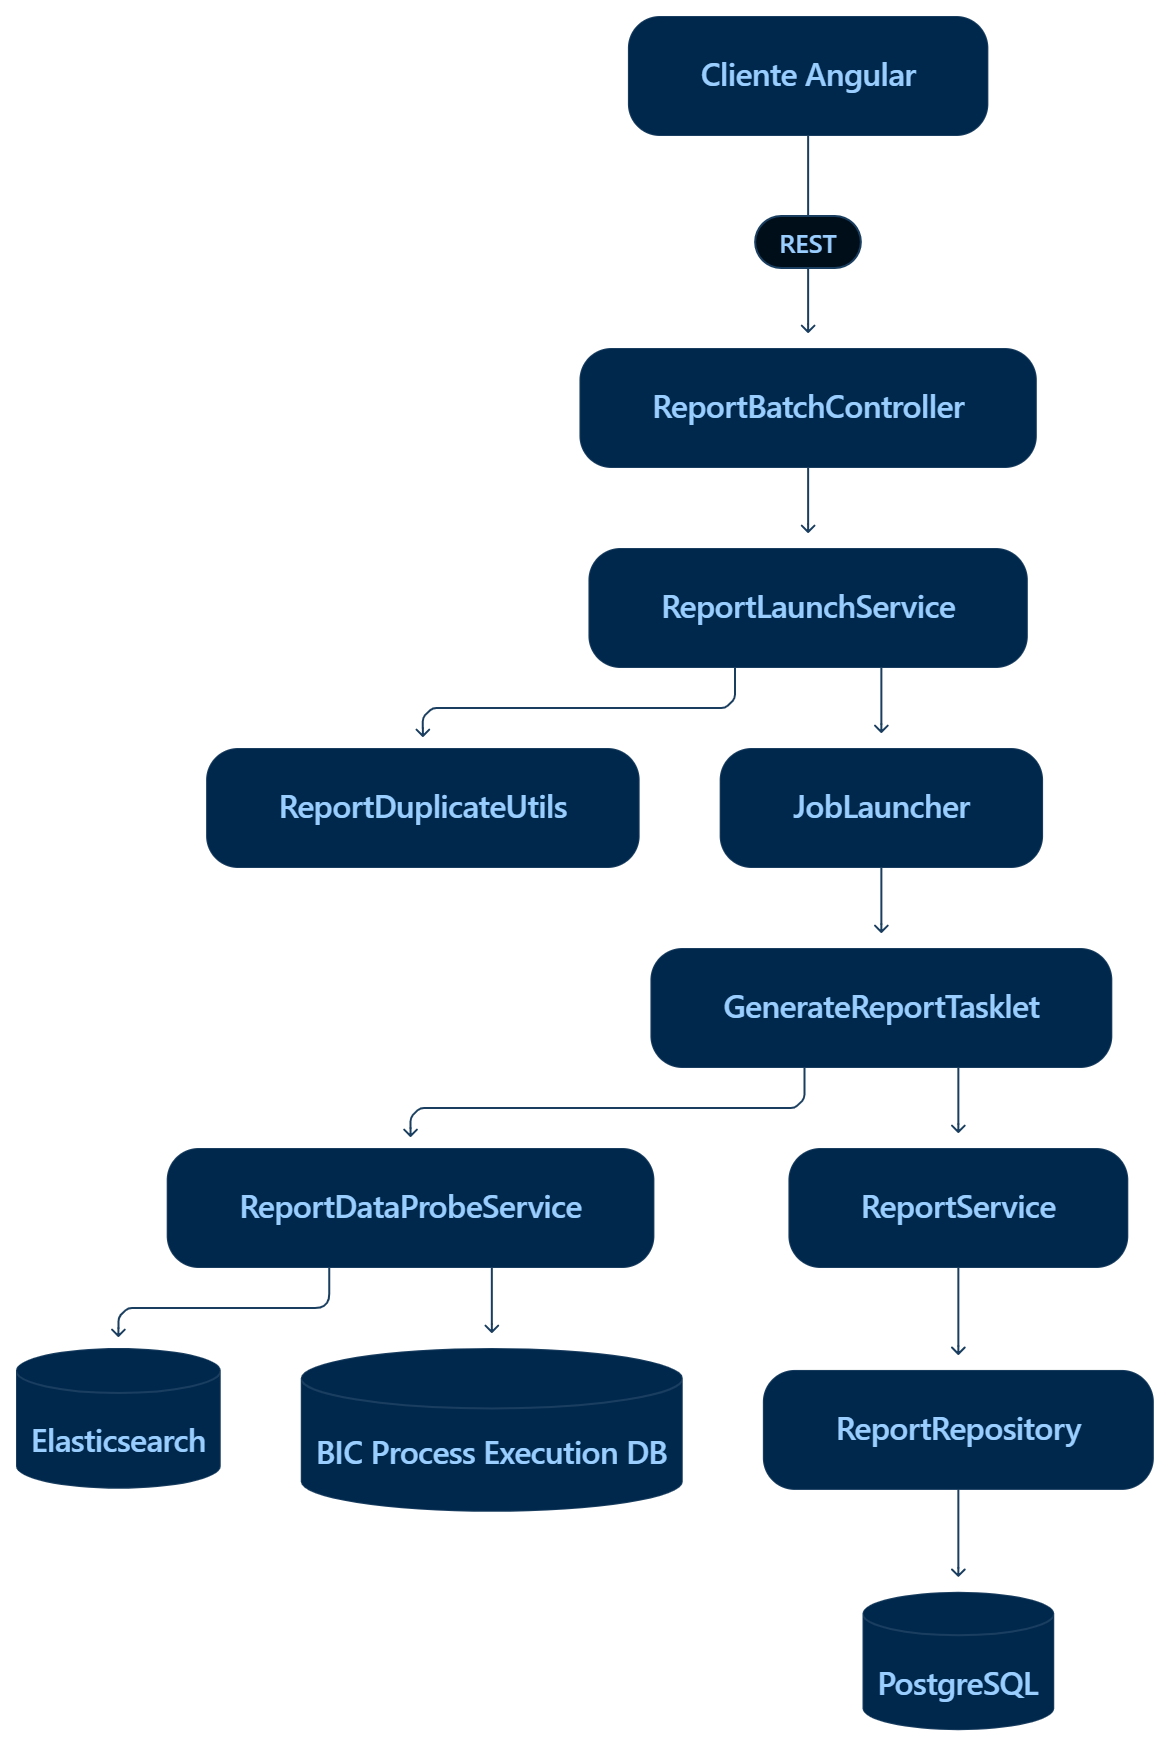
\includegraphics[width=0.90\textwidth]{img/arquitectura_simplificada.png}
  \caption{Arquitectura simplificada del flujo principal de generación de informes. Fuente: elaboración propia.}
  \label{fig:arquitectura-simplificada}
\end{figure}

El cliente Angular envía las solicitudes al backend mediante la API REST
expuesta por \texttt{ReportBatchController}, que delega la coordinación de
una nueva generación en \texttt{ReportLaunchService}.

Antes de iniciar el procesamiento, \texttt{ReportLaunchService} comprueba
mediante \texttt{ReportDuplicateUtils} y \texttt{ReportRepository} si una
solicitud equivalente ha sido desencadenada recientemente. Si no existe
duplicidad, se inicia de forma asíncrona un job de Spring Batch mediante
\texttt{JobLauncher}.

Durante la ejecución del job, \texttt{GenerateReportTasklet} comprueba
mediante \texttt{ReportDataProbeService} que existen datos para los
parámetros solicitados y selecciona el generador correspondiente según el
tipo y la categoría del informe. Una vez construido el workbook, el tasklet
delega su almacenamiento en \texttt{ReportService}, que realiza la
serialización del fichero y utiliza \texttt{ReportRepository} para
persistirlo en PostgreSQL.

La figura del cuerpo principal pretende ofrecer una visión sintética del
flujo de generación. Una representación más completa, que incorpora los
componentes internos del frontend y del backend, las fuentes de datos,
Spring Batch y los elementos de infraestructura y despliegue, se incluye en
el apéndice~\ref{ap:arquitectura-detallada}.

\subsection{Comunicación entre componentes}

La comunicación entre el cliente y el servidor se realiza mediante una
\acrshort{api} \acrshort{rest} sobre \acrshort{http}, utilizando
\acrshort{json} para el intercambio de información estructurada y contenido
binario para la descarga de los ficheros Excel.

Los principales endpoints utilizados son:

\begin{itemize}

  \item \texttt{POST /api/reports}: recibe los parámetros de una nueva
  generación. Antes de iniciar el procesamiento,
  \texttt{ReportLaunchService} comprueba si se ha desencadenado recientemente
  una solicitud equivalente. Si no existe duplicidad, el job se lanza de
  forma asíncrona y la petición queda aceptada para su procesamiento.

  \item \texttt{GET /api/reports/latest}: permite consultar periódicamente
  si el informe correspondiente a una solicitud ya se encuentra disponible.
  Este endpoint constituye la base del mecanismo de \textit{polling}
  utilizado por el frontend.

  \item \texttt{GET /api/reports/history}: devuelve el listado paginado de
  informes almacenados, ordenados de más reciente a más antiguo.

  \item \texttt{GET /api/reports/\{id\}/download}: recupera el contenido
  binario de un informe almacenado a partir de su identificador
  \acrshort{uuid}.

\end{itemize}

La comprobación de disponibilidad de datos no se realiza antes de lanzar el
job, sino durante su ejecución. Una vez iniciado,
\texttt{GenerateReportTasklet} utiliza
\texttt{ReportDataProbeService.hasData()} para determinar si existen datos
para la combinación solicitada. Si no existen, el step finaliza con el estado
\texttt{NO\_DATA} sin construir el fichero Excel.

\subsection{Justificación de la arquitectura elegida}

La arquitectura adoptada responde principalmente a criterios de separación
de responsabilidades, mantenibilidad y desacoplamiento del procesamiento de
larga duración.

\begin{itemize}

  \item \textbf{Modularidad}: cada componente concentra una responsabilidad
  específica. El cliente gestiona la interacción con el usuario; los
  controladores exponen la API; los servicios coordinan la lógica de
  aplicación; y los repositorios encapsulan el acceso a datos.

  \item \textbf{Separación de responsabilidades}: el controlador no contiene
  la lógica específica de construcción de informes. Esta responsabilidad se
  delega en Spring Batch, el tasklet y los servicios especializados de cada
  tipo y categoría de informe.

  \item \textbf{Procesamiento asíncrono}: el uso de Spring Batch y de un
  executor asíncrono permite desacoplar la generación del ciclo principal de
  la petición HTTP, evitando mantener bloqueada la interfaz mientras se
  construye el informe.

  \item \textbf{Persistencia independiente}: la centralización del
  almacenamiento en \texttt{ReportService} y
  \texttt{ReportRepository} permite separar la lógica de generación de la
  forma en que los informes son almacenados y recuperados.

  \item \textbf{Trazabilidad}: Flyway mantiene versionados los cambios en el
  esquema de base de datos, mientras que las tablas de metadatos de Spring
  Batch permiten conservar información sobre las ejecuciones de los jobs.

  \item \textbf{Capacidad de evolución}: la división entre tipos de informe,
  categorías y servicios comunes facilita la incorporación de nuevas
  variantes sin modificar de forma sustancial los puntos de entrada de la
  aplicación.

\end{itemize}

No se realizaron pruebas formales de carga dentro del alcance del proyecto,
por lo que no se pretende cuantificar el comportamiento del sistema ante
niveles elevados de concurrencia. La arquitectura sí proporciona una base
desacoplada sobre la que podrían estudiarse futuras mejoras de capacidad y
escalabilidad.

\subsection{Stack tecnológico}

El stack tecnológico final utilizado se compone de:

\begin{itemize}

  \item \textbf{Cliente}: Angular 15, TypeScript, Angular Material, RxJS y
  Yarn.

  \item \textbf{Servidor}: Spring Boot 3, Spring Batch, Hibernate/JPA y
  Maven.

  \item \textbf{Almacenamiento}: PostgreSQL para los informes y sus
  metadatos, y Elasticsearch como una de las fuentes de información de los
  procesos.

  \item \textbf{Generación de Excel}: Aspose Cells para la construcción y el
  formato de los workbooks.

  \item \textbf{Migraciones}: Flyway para el control de versiones del
  esquema de base de datos.

  \item \textbf{Infraestructura}: Docker para contenerización y
  Ansible/AWX para automatización del despliegue.

\end{itemize}


%%%%%%%%%%%%%%%%%%%%%%%%%%%%%%%%%%%%%%%%%
% Diseño de la aplicación              %
%%%%%%%%%%%%%%%%%%%%%%%%%%%%%%%%%%%%%%%%%

\section{Diseño de la aplicación}

A continuación se detalla el diseño interno de los principales componentes
del sistema, describiendo la organización del cliente y del servidor, el
flujo de generación y la capa de persistencia.

\subsection{Cliente}

El cliente web se organiza mediante componentes y servicios Angular que
separan la presentación de la comunicación con el backend.

\subsubsection{Estructura de módulos y componentes}

El frontend del proyecto está ubicado en
\texttt{webapp/custom-aesla-angular-front}. La organización relevante dentro
de \texttt{src/app} es la siguiente:

\begin{itemize}

  \item \textbf{\texttt{reports-generator}}: contiene el componente principal
  de generación de informes.

  \begin{itemize}
    \item \texttt{reports-generator.component.ts}: lógica del componente.
    \item \texttt{reports-generator.component.html}: plantilla del formulario.
    \item \texttt{reports-generator.component.scss}: estilos específicos.
    \item \texttt{reports-generator.component.spec.ts}: pruebas unitarias.
  \end{itemize}

  \item \textbf{\texttt{reports-history}}: agrupa el componente encargado del
  historial y de su tabla paginada.

  \begin{itemize}
    \item \texttt{reports-history.component.ts}: lógica del componente.
    \item \texttt{reports-history.component.html}: plantilla de la tabla.
    \item \texttt{reports-history.component.scss}: estilos del historial.
    \item \texttt{reports-history.component.spec.ts}: pruebas unitarias.
    \item \texttt{dialog/}: diálogos auxiliares utilizados por la interfaz.
  \end{itemize}

  \item \textbf{\texttt{services}}: contiene los servicios responsables de
  la comunicación HTTP con el backend.

  \begin{itemize}
    \item \texttt{get-alternative-franchise-list.service.ts}.
    \item \texttt{get-innovation-franchise-list.service.ts}.
    \item \texttt{report-download.service.ts}.
    \item \texttt{reports-history.service.ts}.
  \end{itemize}

  \item \textbf{Archivos raíz}:

  \begin{itemize}
    \item \texttt{app.component.ts}: componente raíz.
    \item \texttt{app.module.ts}: módulo principal.
    \item \texttt{app-routing.module.ts}: configuración de las rutas entre
    generación e historial.
  \end{itemize}

\end{itemize}

Esta organización mantiene separadas las principales responsabilidades del
cliente: el componente de generación gestiona la creación de informes, el
historial permite consultar y redescargar los existentes y los servicios
centralizan las comunicaciones con el backend.

\subsubsection{Servicios Angular}

Los servicios encapsulan las peticiones HTTP y la gestión de las respuestas
recibidas desde el backend.

\begin{itemize}

  \item \textbf{\texttt{get-alternative-franchise-list.service.ts}}:
  obtiene las franquicias disponibles para informes de categoría
  Alternativa.

  \item \textbf{\texttt{get-innovation-franchise-list.service.ts}}:
  realiza la misma función para la categoría Innovación.

  \item \textbf{\texttt{report-download.service.ts}}:
  gestiona el flujo de generación y descarga. Entre sus responsabilidades se
  encuentran:

  \begin{itemize}
    \item enviar la petición \texttt{POST /api/reports};
    \item realizar el seguimiento de la generación mediante
    \textit{polling};
    \item solicitar la descarga una vez disponible el informe;
    \item recibir el fichero Excel como contenido binario;
    \item gestionar los mensajes de estado y situaciones de error.
  \end{itemize}

  \item \textbf{\texttt{reports-history.service.ts}}:
  centraliza las operaciones relacionadas con el historial.

  \begin{itemize}
    \item \texttt{getHistory(page, size)} obtiene el listado paginado mediante
    \texttt{GET /api/reports/history}.
    \item \texttt{downloadReport(id)} recupera un informe almacenado mediante
    \texttt{GET /api/reports/\{id\}/download}.
    \item transforma las respuestas recibidas a los modelos TypeScript
    utilizados por los componentes.
  \end{itemize}

\end{itemize}

Los servicios utilizan \texttt{HttpClient} para las peticiones HTTP y
Observables de RxJS para la gestión de los flujos asíncronos. Asimismo,
utilizan el mecanismo de inyección de dependencias de Angular mediante
\texttt{@Injectable}.

\subsubsection{Flujo de datos entre componentes}

El flujo habitual de generación de un informe puede resumirse en los
siguientes pasos:

\begin{enumerate}

  \item El usuario configura en \texttt{ReportsGeneratorComponent} el tipo,
  la categoría, las franquicias y, cuando procede, el rango de fechas.

  \item Al seleccionar una categoría se consulta dinámicamente la lista de
  franquicias mediante el servicio correspondiente.

  \item Al pulsar el botón de generación, el componente valida los parámetros
  introducidos.

  \item Si los parámetros son válidos,
  \texttt{ReportDownloadService} envía una petición
  \texttt{POST /api/reports}.

  \item El backend comprueba mediante
  \texttt{ReportDuplicateUtils} y el repositorio si se ha desencadenado una
  solicitud equivalente dentro de la ventana temporal definida.

  \item Si se detecta una duplicidad, no se inicia un nuevo job y se informa
  al usuario de la existencia de una solicitud reciente.

  \item Si la solicitud puede procesarse,
  \texttt{ReportLaunchService} inicia de forma asíncrona el job de Spring
  Batch y el cliente comienza el seguimiento del resultado.

  \item Durante la ejecución del job,
  \texttt{GenerateReportTasklet} utiliza
  \texttt{ReportDataProbeService} para comprobar si existen datos. Si no
  existen, el procesamiento finaliza con el estado
  \texttt{NO\_DATA}.

  \item Mientras la generación continúa,
  \texttt{ReportDownloadService} consulta periódicamente
  \texttt{/api/reports/latest}. En la implementación utilizada, la consulta
  se realiza cada cinco segundos durante un máximo de 120 segundos.

  \item Cuando el informe se encuentra disponible, la respuesta incluye su
  identificador y el cliente solicita
  \texttt{/api/reports/\{id\}/download}, recibe el contenido como
  \textit{blob} y comienza la descarga.

  \item Independientemente de la descarga inmediata, el informe queda
  almacenado y puede recuperarse posteriormente desde
  \texttt{ReportsHistoryComponent}.

\end{enumerate}

\subsubsection{Validaciones y feedback al usuario}

El formulario de generación aplica validaciones antes de enviar la solicitud:

\begin{itemize}

  \item tipo y categoría de informe obligatorios;
  \item selección de al menos una franquicia;
  \item comprobación de coherencia del rango de fechas cuando este se
  especifica;
  \item presentación de mensajes asociados a errores de validación.

\end{itemize}

Durante el proceso, la interfaz muestra mensajes relacionados con las
distintas situaciones del flujo, como la comprobación de la solicitud, el
inicio de la generación, la disponibilidad del fichero, la existencia de un
informe reciente o los errores producidos.

El seguimiento no se realiza mediante una conexión persistente entre cliente
y servidor. El frontend consulta periódicamente
\texttt{/api/reports/latest}, por lo que el mecanismo utilizado corresponde a
\textit{polling} y no a una comunicación mediante WebSocket o Server-Sent
Events.

\subsubsection{Frameworks y librerías de interfaz}

El cliente utiliza principalmente:

\begin{itemize}

  \item \textbf{Angular Material}: biblioteca de componentes de interfaz que
  proporciona formularios, tablas, botones, diálogos y
  \textit{snackbars}~\cite{AngularMaterialDocs}.

  \item \textbf{RxJS}: biblioteca empleada para trabajar con flujos
  asíncronos mediante Observables~\cite{RxJSDocs}.

  \item \textbf{Yarn}: gestor utilizado para la instalación y resolución de
  las dependencias del frontend.

\end{itemize}


%%%%%%%%%%%%%%%%%%%%%%%%%%%%%%%%%%%%%%%%%
% Servidor                              %
%%%%%%%%%%%%%%%%%%%%%%%%%%%%%%%%%%%%%%%%%

\subsection{Servidor (Spring Boot + Spring Batch)}

El backend sigue una organización modular en capas, utilizando el mecanismo
de inyección de dependencias proporcionado por Spring. El código separa la
configuración, los puntos de entrada REST, la coordinación del procesamiento,
la lógica específica de cada tipo de informe y la persistencia.

\subsubsection{Estructura de paquetes}

El backend está ubicado en
\texttt{main/java/com/gbtec/bic/cloud}. Los paquetes más relevantes para el
Report Service son:

\begin{itemize}

  \item \textbf{\texttt{config}}: configuración general de Spring.

  \begin{itemize}
    \item \texttt{AsposeConfiguration}: configuración de Aspose Cells.
    \item \texttt{WebSecurityConfig}: configuración de seguridad web y CORS.
  \end{itemize}

  \item \textbf{\texttt{datastorage.elasticsearch}}:
  integración con Elasticsearch.

  \begin{itemize}
    \item \texttt{ElasticsearchService}: servicio utilizado para consultar
    variables de procesos.
  \end{itemize}

  \item \textbf{\texttt{processes.batch}}:
  infraestructura relacionada con Spring Batch.

  \begin{itemize}
    \item \texttt{BatchAsyncConfiguration}: configuración del executor
    asíncrono.
    \item \texttt{ReportBatchConfig}: definición del job y de su step.
    \item \texttt{FranchiseController}: endpoints relacionados con
    franquicias.
    \item \texttt{ReportBatchController}: endpoints de generación y consulta
    de informes.
    \item \texttt{ReportParamService}: preparación de parámetros del job.
    \item \texttt{ReportRequestDto}: representación de la solicitud.
    \item \texttt{GenerateReportTasklet}: ejecución de la generación.
    \item \texttt{ReportDuplicateUtils}: cálculo de la firma y comprobación
    de duplicidad.
    \item \texttt{ReportFileNameUtils}: construcción de nombres de fichero.
    \item \texttt{ReportParamUtils}: normalización y tratamiento de
    parámetros.
  \end{itemize}

  \item \textbf{\texttt{kpi\_reports}}:
  lógica específica para informes KPI, organizada por las categorías
  \texttt{alternative} e \texttt{innovation}. Cada categoría contiene sus
  modelos, repositorios, servicios y utilidades correspondientes.

  \item \textbf{\texttt{product\_reports}}:
  lógica específica para los informes de Producto, también separada entre
  \texttt{alternative} e \texttt{innovation}, con componentes de acceso a
  datos y generación.

  \item \textbf{\texttt{report\_probe}}:
  funcionalidad de comprobación de disponibilidad de datos y coordinación del
  lanzamiento.

  \begin{itemize}
    \item \texttt{ReportDataProbeService}.
    \item \texttt{ReportDataProbeServiceImpl}.
    \item \texttt{ReportLaunchService}.
  \end{itemize}

  \item \textbf{\texttt{report\_storage}}:
  persistencia de los informes.

  \begin{itemize}
    \item \texttt{ReportEntity}.
    \item \texttt{ReportRepository}.
    \item \texttt{ReportService}.
  \end{itemize}

  \item \textbf{\texttt{utils}}:
  utilidades compartidas relacionadas principalmente con la construcción y el
  formato de los libros Excel.

  \begin{itemize}
    \item \texttt{heatmap/}.
    \item \texttt{CreateExcelFileUtils}.
    \item \texttt{ExcelCellStyleUtils}.
  \end{itemize}

  \item \textbf{\texttt{ui}}:
  configuración y controladores utilizados para servir la interfaz.

\end{itemize}

Esta organización separa la configuración del procesamiento batch, la lógica
específica de los informes, la comprobación de datos, la persistencia y las
utilidades comunes.

En particular, \texttt{BatchAsyncConfiguration} configura el executor
asíncrono y \texttt{ReportBatchConfig} define el job y el step de generación.
\texttt{ReportBatchController} actúa como punto de entrada REST, mientras que
\texttt{ReportRequestDto} agrupa los parámetros necesarios para identificar
el tipo de informe, la categoría, las franquicias y las fechas opcionales.

\subsubsection{Patrones y principios de diseño}

El backend aplica varios mecanismos habituales del ecosistema Spring:

\begin{itemize}

  \item \textbf{Arquitectura en capas}: separación entre controladores,
  servicios y repositorios.

  \item \textbf{Inyección de dependencias}: Spring gestiona las dependencias
  entre componentes y su ciclo de vida.

  \item \textbf{DTO}: los parámetros de la generación se agrupan en
  \texttt{ReportRequestDto}, evitando acoplar la representación externa de
  las solicitudes a las entidades de persistencia.

  \item \textbf{Delegación de responsabilidades}: el controlador no genera
  directamente los informes, sino que delega la coordinación en los
  servicios y la ejecución en Spring Batch.

\end{itemize}

\subsubsection{Organización de los generadores de informes}

La lógica de generación se divide en dos ramas principales:
\texttt{kpi\_reports} y \texttt{product\_reports}. Cada una se divide a su vez
entre las categorías \texttt{alternative} e \texttt{innovation}.

Esta separación es necesaria porque los informes KPI y Producto trabajan con
modelos de datos y métricas diferentes.

En los informes KPI, los servicios correspondientes recuperan las instancias
y los proyectos necesarios, calculan indicadores y generan las hojas
específicas del workbook.

En los informes de Producto, los componentes de acceso a datos recuperan la
información necesaria para construir elementos como retroplannings, informes
diarios y heatmaps.

Las operaciones compartidas relacionadas con estilos, creación de celdas y
formato del libro se concentran en las utilidades comunes de Excel.

La selección del generador puede representarse de forma simplificada de la
siguiente manera:

\begin{lstlisting}[caption={Selección del generador según los parámetros del informe}]
if type == PRODUCT and category == ALTERNATIVE:
  generate product alternative report
else if type == PRODUCT and category == INNOVATION:
  generate product innovation report
else if type == KPI and category == ALTERNATIVE:
  generate KPI alternative report
else if type == KPI and category == INNOVATION:
  generate KPI innovation report
else:
  reject invalid configuration
\end{lstlisting}

\subsubsection{Flujo de generación de informes}

El flujo completo de generación es el siguiente:

\begin{enumerate}

  \item \texttt{ReportBatchController} recibe la petición
  \texttt{POST /api/reports}.

  \item El controlador recibe los parámetros mediante
  \texttt{ReportRequestDto} y delega la coordinación en
  \texttt{ReportLaunchService}.

  \item \texttt{ReportLaunchService} comprueba la posible duplicidad:

  \begin{itemize}

    \item \texttt{ReportDuplicateUtils} genera la firma asociada a la
    solicitud.

    \item mediante el repositorio se comprueba si se ha desencadenado
    recientemente una solicitud con los mismos parámetros;

    \item si existe una solicitud equivalente dentro de la ventana definida,
    no se inicia un nuevo job;

    \item en caso contrario, se continúa con el lanzamiento.

  \end{itemize}

  \item \texttt{ReportLaunchService} utiliza \texttt{JobLauncher} para
  iniciar de forma asíncrona el job definido en Spring Batch.

  \item El job contiene un único step implementado mediante
  \texttt{GenerateReportTasklet}.

  \item Al comenzar la ejecución,
  \texttt{GenerateReportTasklet} extrae los parámetros del job y llama a
  \texttt{ReportDataProbeService.hasData()}.

  \item Si no existen datos para la combinación solicitada, el step finaliza
  con el estado \texttt{NO\_DATA} sin construir el workbook.

  \item Si existen datos, el tasklet selecciona el generador correspondiente
  según el tipo y la categoría del informe.

  \item Los servicios especializados obtienen la información necesaria desde
  BIC Process Execution y Elasticsearch, realizan las transformaciones y
  cálculos y construyen el workbook utilizando Aspose Cells y las utilidades
  comunes.

  \item Una vez construido el fichero,
  \texttt{GenerateReportTasklet} delega su almacenamiento en
  \texttt{ReportService}.

  \item \texttt{ReportService} serializa el workbook, construye la entidad y
  utiliza \texttt{ReportRepository} para almacenar los metadatos y el
  contenido binario en PostgreSQL.

  \item El informe queda disponible para ser detectado mediante
  \texttt{/api/reports/latest}, descargado mediante su identificador y
  consultado posteriormente desde el historial.

\end{enumerate}

La lógica principal puede resumirse mediante el siguiente pseudocódigo:

\begin{lstlisting}[caption={Pseudocódigo de la solicitud y generación de un informe}]
requestGeneration(request):
  if reportDuplicateUtils.wasTriggeredRecently(request):
    return DUPLICATE

  jobId = reportLaunchService.launch(request)
  return STARTED(jobId)


execute(stepContribution, jobParameters):
  if not reportDataProbe.hasData(jobParameters):
    stepContribution.setExitStatus(NO_DATA)
    return FINISHED

  workbook = generateWorkbook(jobParameters)
  reportService.store(workbook)

  return FINISHED
\end{lstlisting}

De este modo, \texttt{ReportLaunchService} coordina la comprobación de
duplicidad y el lanzamiento del job, mientras que la disponibilidad de datos
forma parte del propio flujo de ejecución y es comprobada por
\texttt{GenerateReportTasklet}. Esta separación evita introducir en el
controlador lógica específica de cada tipo de informe.

\subsubsection{Comprobación de disponibilidad de datos}

\texttt{ReportDataProbeService} permite determinar si existen datos
suficientes para generar el informe antes de ejecutar toda la lógica de
construcción del workbook.

Su implementación,
\texttt{ReportDataProbeServiceImpl}, selecciona la estrategia de comprobación
según el tipo y la categoría del informe.

Para los informes de Producto, se normalizan previamente las franquicias y
las fechas mediante \texttt{ReportParamUtils}. En la categoría Alternativa
se utiliza \texttt{AlternativeExportDataService}, mientras que para
Innovación se utiliza \texttt{InnovationExportDataService}. Se considera que
no existen datos cuando los procesos recuperados no contienen tareas
relevantes.

Para KPI, las franquicias se transforman al formato esperado y se utiliza
\texttt{KpiAlternativeInstanceService} o
\texttt{KpiInnovationInstanceService} según la categoría. La comprobación se
basa en la existencia de proyectos asociados a las franquicias solicitadas.

De forma simplificada:

\begin{lstlisting}[caption={Comprobación de disponibilidad de datos}]
hasData(type, category, franchises, startDate, endDate):
  if type == PRODUCT:
    normalize parameters and dates
    data = load PRODUCT data for category
    return data contains at least one task

  if type == KPI:
    franchiseList = parse franchises
    data = load KPI projects for category
    return data contains at least one project

  raise invalid report type
\end{lstlisting}

\subsubsection{Diseño del Job y Step de Spring Batch}

El job de generación se define en \texttt{ReportBatchConfig} y utiliza:

\begin{itemize}

  \item \textbf{Parámetros del job}: tipo, categoría, franquicias, fechas y
  los identificadores necesarios para la ejecución.

  \item \textbf{Un único Step}: implementado mediante
  \texttt{GenerateReportTasklet}.

  \item \textbf{Executor asíncrono}: configurado en
  \texttt{BatchAsyncConfiguration}, permitiendo que el job se ejecute sin
  bloquear el thread encargado de responder a la petición HTTP.

\end{itemize}

Se optó por un \textit{Tasklet} en lugar del modelo
\texttt{ItemReader}--\texttt{ItemProcessor}--\texttt{ItemWriter}, ya que la
generación de cada informe constituye una operación completa que combina la
obtención de información, el cálculo de métricas y la construcción de un
workbook complejo.

Spring Batch proporciona además las tablas de metadatos necesarias para
registrar las instancias, ejecuciones, parámetros y estados asociados a los
jobs y steps.

Una vez generada la información,
\texttt{GenerateReportTasklet} no accede directamente al repositorio. El
almacenamiento se delega en \texttt{ReportService}, que centraliza la
conversión del workbook a bytes, la construcción de la entidad y su
persistencia mediante \texttt{ReportRepository}.

Esta decisión evita repetir el proceso de serialización y almacenamiento en
cada uno de los generadores de informes.


%%%%%%%%%%%%%%%%%%%%%%%%%%%%%%%%%%%%%%%%%
% Capa de datos                         %
%%%%%%%%%%%%%%%%%%%%%%%%%%%%%%%%%%%%%%%%%

\subsection{Capa de datos}

La capa de persistencia almacena los informes generados junto con la
información necesaria para identificarlos, consultarlos y descargarlos
posteriormente.

\subsubsection{Modelo de persistencia}

El esquema \texttt{aesla\_reports} contiene una única tabla principal
\texttt{report}, gestionada mediante migraciones de Flyway. La entidad JPA
\texttt{ReportEntity} representa esta tabla.

Los principales atributos son:

\begin{itemize}

  \item \texttt{id} (UUID): identificador único.
  \item \texttt{file\_name} (String): nombre del fichero Excel.
  \item \texttt{report\_type} (enum): KPI o PRODUCT.
  \item \texttt{report\_category} (enum): INNOVATION o ALTERNATIVE.
  \item \texttt{created\_at} (LocalDateTime): fecha y hora de creación.
  \item \texttt{start\_date} y \texttt{end\_date} (LocalDate): rango de
  fechas opcional.
  \item \texttt{franchises} (String): franquicias asociadas.
  \item \texttt{file\_size} (Long): tamaño del fichero.
  \item \texttt{content} (byte[]): contenido binario del workbook.
\end{itemize}

\subsubsection{Justificación del esquema y uso de Flyway}

Se utiliza un esquema específico, \texttt{aesla\_reports}, para mantener los
datos del Report Service separados del resto de los esquemas utilizados por
la plataforma.

Flyway permite:

\begin{itemize}

  \item versionar los cambios del esquema mediante scripts
  \acrshort{sql};
  \item aplicar únicamente las migraciones todavía no ejecutadas;
  \item mantener trazabilidad mediante
  \texttt{flyway\_schema\_history};
  \item integrar el proceso de migración con el arranque de Spring Boot.
\end{itemize}

La configuración desarrollada contempla tres grupos principales de
migraciones. En primer lugar se crea el esquema
\texttt{aesla\_reports}; posteriormente se crea la tabla
\texttt{report}; finalmente se incorporan las tablas de metadatos requeridas
por Spring Batch.

Entre estas últimas se encuentran:

\begin{itemize}
  \item \texttt{BATCH\_JOB\_INSTANCE};
  \item \texttt{BATCH\_JOB\_EXECUTION};
  \item \texttt{BATCH\_JOB\_EXECUTION\_PARAMS};
  \item \texttt{BATCH\_STEP\_EXECUTION};
  \item \texttt{BATCH\_JOB\_EXECUTION\_CONTEXT};
  \item \texttt{BATCH\_STEP\_EXECUTION\_CONTEXT}.
\end{itemize}

Estas tablas permiten a Spring Batch identificar las instancias de los jobs,
registrar sus ejecuciones y mantener los parámetros y contextos asociados.

La configuración correspondiente se encuentra en
\texttt{application.yaml}, donde se definen las propiedades relacionadas con
JPA, JDBC, Flyway y la infraestructura de Spring Batch. El objetivo es
garantizar que las estructuras necesarias se encuentren disponibles antes de
iniciar cualquier job.

\texttt{ReportRepository} extiende \texttt{JpaRepository} y encapsula el
acceso a los informes almacenados. Sobre él,
\texttt{ReportService} implementa la lógica asociada a la persistencia y
recuperación: serializa el workbook, construye la entidad, ejecuta la
operación \texttt{save} y recupera los informes cuando son solicitados por
identificador o por los criterios correspondientes.

\setlength{\tabcolsep}{1pt}%
\renewcommand{\arraystretch}{1.15}%

{\small
\rowcolors{3}{udcgray!08}{white}

\begin{longtable}{@{} p{0.19\textwidth} p{0.24\textwidth} p{0.07\textwidth} p{0.45\textwidth} @{}}

\caption{Atributos de la entidad \textit{Report} en \textit{aesla\_reports.report}.}
\label{tab:modelo-informe-design}\\

\toprule
\rowcolor{udcpink!20}
\textbf{Campo (columna)} &
\textbf{Tipo lógico (Java / SQL)} &
\textbf{Nulo} &
\textbf{Descripción} \\
\midrule
\endfirsthead

\multicolumn{4}{r}{\small\itshape (continúa de la página anterior)}\\
\toprule
\rowcolor{udcpink!20}
\textbf{Campo (columna)} &
\textbf{Tipo lógico (Java / SQL)} &
\textbf{Nulo} &
\textbf{Descripción} \\
\midrule
\endhead

\midrule
\multicolumn{4}{r}{\small\itshape (continúa en la siguiente página)}\\
\endfoot

\bottomrule
\endlastfoot

\texttt{id} &
UUID / UUID &
No &
Identificador único del informe (clave primaria).\\

\texttt{file\_name} &
String / varchar(512) &
No &
Nombre del fichero Excel generado.\\

\texttt{report\_type} &
enum ReportType / varchar &
No &
Tipo de informe: \texttt{KPI} o \texttt{PRODUCT}.\\

\texttt{report\_category} &
enum ReportCategory / varchar &
No &
Categoría: \texttt{INNOVATION} o \texttt{ALTERNATIVE}.\\

\texttt{created\_at} &
LocalDateTime / timestamp &
No &
Fecha y hora de creación.\\

\texttt{start\_date} &
LocalDate / date &
Sí &
Fecha inicial del rango solicitado.\\

\texttt{end\_date} &
LocalDate / date &
Sí &
Fecha final del rango solicitado.\\

\texttt{franchises} &
String / text &
No &
Franquicia o conjunto de franquicias seleccionadas.\\

\texttt{file\_size} &
Long / bigint &
No &
Tamaño del fichero en bytes.\\

\texttt{content} &
byte[] / bytea &
No &
Contenido binario del workbook.\\

\end{longtable}

\rowcolors{2}{}{}
}


%%%%%%%%%%%%%%%%%%%%%%%%%%%%%%%%%%%%%%%%%
% Interacción cliente-servidor         %
%%%%%%%%%%%%%%%%%%%%%%%%%%%%%%%%%%%%%%%%%

\section{Interacción cliente--servidor}

Esta sección concreta las operaciones intercambiadas entre el cliente Angular
y el backend Spring Boot a través de la API REST.

\subsection{Endpoints REST}

\subsubsection{Inicio de una generación}

El endpoint:

\begin{center}
\texttt{POST /api/reports}
\end{center}

recibe los parámetros necesarios para iniciar una nueva generación. Un cuerpo
de petición simplificado puede representarse de la siguiente manera:

\begin{lstlisting}[caption={Ejemplo de solicitud de generación en JSON}]
{
  "reportType": "KPI",
  "reportCategory": "INNOVATION",
  "franchises": ["Starbucks", "Vips"],
  "startDate": "2024-01-01",
  "endDate": "2024-12-31"
}
\end{lstlisting}

La operación realiza las validaciones iniciales y la comprobación de
duplicidad. Cuando la solicitud puede procesarse, se inicia el job asíncrono
y se devuelve al cliente la confirmación de que la generación ha comenzado.

La ausencia de datos puede detectarse posteriormente durante la ejecución del
tasklet, por lo que el cliente utiliza el mecanismo de seguimiento para
conocer el resultado final.

\subsubsection{Consulta del historial}

El endpoint:

\begin{center}
\texttt{GET /api/reports/history?page=0\&size=5}
\end{center}

devuelve una página del historial de informes.

Una respuesta simplificada es:

\begin{lstlisting}[caption={Ejemplo de respuesta paginada en JSON}]
{
  "content": [
    {
      "id": "uuid",
      "fileName": "KPI_Innovation_2024-11-15.xlsx",
      "reportType": "KPI",
      "reportCategory": "INNOVATION",
      "createdAt": "2024-11-15T10:30:00",
      "franchises": "Starbucks,Vips",
      "fileSize": 1048576
    }
  ],
  "totalElements": 42,
  "totalPages": 9,
  "number": 0
}
\end{lstlisting}

\subsubsection{Seguimiento de la generación}

El endpoint:

\begin{center}
\texttt{GET /api/reports/latest}
\end{center}

se utiliza durante el mecanismo de \textit{polling} para comprobar si el
informe solicitado ya se encuentra disponible. El cliente realiza consultas
periódicas hasta obtener la confirmación de disponibilidad o alcanzar el
tiempo máximo de espera configurado.

\subsubsection{Descarga de un informe}

El endpoint:

\begin{center}
\texttt{GET /api/reports/\{id\}/download}
\end{center}

recupera un informe almacenado a partir de su identificador. Cuando el
informe existe, el servidor devuelve su contenido binario en formato Excel;
si el identificador no corresponde a ningún informe almacenado, la operación
devuelve el error correspondiente.

\subsection{Manejo de errores}

La API utiliza códigos \acrshort{http} estándar para representar el resultado
de las operaciones. Entre los principales casos contemplados se encuentran:

\begin{itemize}

  \item \textbf{200 OK}: consulta o descarga realizada correctamente.

  \item \textbf{202 Accepted}: petición aceptada para procesamiento
  asíncrono, cuando este código es utilizado por la implementación del
  controlador.

  \item \textbf{400 Bad Request}: parámetros de entrada inválidos.

  \item \textbf{409 Conflict}: existencia de una solicitud equivalente
  reciente cuando la duplicidad se representa mediante este código.

  \item \textbf{404 Not Found}: no existe el informe solicitado.

  \item \textbf{500 Internal Server Error}: error no controlado durante el
  procesamiento.

\end{itemize}

Cuando corresponde, las respuestas de error incluyen información estructurada
que permite al cliente identificar la situación y mostrar un mensaje
comprensible al usuario. Por ejemplo:

\begin{lstlisting}[caption={Ejemplo simplificado de una respuesta de error}]
{
  "error": "DUPLICATE_REPORT",
  "message": "Un informe idéntico fue generado recientemente.",
  "reportId": "uuid"
}
\end{lstlisting}

%%%%%%%%%%%%%%%%%%%%%%%%%%%%%%%%%%%%%%%%%
 % Capítulo   6                         %
 %%%%%%%%%%%%%%%%%%%%%%%%%%%%%%%%%%%%%%%%

\chapter{Implementación y pruebas}

\section{Tareas de mejora}

Durante el desarrollo del proyecto, se abordaron diversas tareas de mejora que no solo añadieron nuevas funcionalidades, sino que también optimizaron la calidad, seguridad y mantenibilidad del código existente. Estas tareas se clasificaron en diferentes categorías según su naturaleza y prioridad, y se gestionaron a través del sistema de seguimiento Jira como parte del \acrshort{epic} "Improvements for AESLA Project in 2025 Q3 \& Q4".\\  

Las tareas de mejora se distribuyeron a lo largo de los tres meses, abordando aspectos críticos como la seguridad de las dependencias, la cobertura de pruebas, la refactorización del código, la observabilidad y la incorporación de nuevas funcionalidades. A continuación, se describen en detalle las principales categorías de tareas de mejora abordadas durante el proyecto.

\subsection{Organización de los work items}

El trabajo se organizó en Jira mediante el EPIC \textit{Improvements for AESLA Project in 2025 Q3 \& Q4}. Este elemento actuó como padre común de los work items relacionados con la evolución del Report Service. La mayoría fueron tareas técnicas, aunque también se registraron incidencias de tipo \textit{Bug} y una historia de usuario de prioridad alta que concentró la introducción del procesamiento asíncrono con Spring Batch.

Cada work item se desarrolló en una rama independiente identificada con su número. En ella se realizaron los commits y, al finalizar, se abrió un Pull Request hacia \texttt{development}. El cambio se integraba después de superar la revisión de código y las comprobaciones de calidad y QA. Todos los elementos compartían la misma \textit{fix version} del Report Service, facilitando la trazabilidad de los cambios incluidos en la publicación.

Entre los trabajos realizados se incluyeron la reducción de duplicación, el aumento de cobertura, la persistencia y consulta de informes, la generación asíncrona, la incorporación de logs, la mejora de las páginas de generación e historial y la resolución de problemas de inicialización de Spring Batch.

\subsection{Persistencia y consulta de informes}

Una de las tareas principales consistió en permitir que los informes generados se almacenaran en la base de datos y pudieran descargarse posteriormente desde el historial. Aunque se gestionó como una tarea técnica, se especificó mediante una historia de usuario: un usuario debía poder acceder a la página de historial, consultar los informes generados y descargar de nuevo cualquiera de ellos.

La implementación se dividió en varias subtareas: creación del esquema de base de datos, integración de su gestión mediante Flyway, creación del repositorio para recuperar el contenido y los metadatos, y refactorización del tratamiento de franquicias y fechas en los informes de Producto y KPI para utilizar una aproximación común. La información almacenada incluye la fecha y hora de generación, el nombre y tamaño del fichero, su contenido y los datos necesarios para identificar la configuración utilizada.

\subsection{Vulnerabilidades}

El \textit{frontend} presentaba inicialmente múltiples vulnerabilidades (\acrshort{cve}) asociadas a sus dependencias. En un primer momento, el origen del problema se debía en parte a la coexistencia de los gestores de paquetes \textit{npm} y \textit{Yarn}, lo que generaba inconsistencias en el árbol de dependencias y diferentes resoluciones de versiones según el gestor empleado. Una vez unificada la gestión en \textit{Yarn}, las vulnerabilidades no desaparecieron por completo, ya que la versión de \textit{Angular} utilizada (15) era considerablemente anterior, lo que limitaba el acceso a versiones parcheadas de algunas librerías, tal y como se recoge en la documentación técnica.\\

\textbf{Estrategia adoptada}: 

\begin{enumerate}
    \item \textbf{Estandarización en Yarn}: se eliminaron los ficheros \texttt{package-lock.json}, se configuró \textit{Yarn} como gestor único en los archivos \texttt{angular.json} y \texttt{package.json}, y se realizó un proceso de deduplicación con \texttt{yarn-deduplicate} seguido de una reinstalación completa de dependencias. Esta medida permitió estabilizar el entorno de desarrollo y homogeneizar la instalación en local y en \acrshort{ci}.
    
    \item \textbf{Mitigación mediante \texttt{resolutions}}: dado que la actualización a una versión posterior de Angular con soporte vigente quedaba fuera del alcance del proyecto, se optó por emplear el bloque \texttt{resolutions} de \textit{Yarn} para forzar versiones parcheadas de dependencias transitivas, sobrescribiendo las versiones vulnerables solicitadas por los paquetes padre. Esta técnica permitió corregir gran parte de los avisos de seguridad sin alterar el núcleo del framework.
\end{enumerate}

\textbf{Situación final}: tras la estandarización y las \texttt{resolutions}, el número de vulnerabilidades se redujo significativamente, quedando solo tres \textit{CVEs} menores vinculadas a dependencias del tooling de \textit{Angular}. Dado que su impacto era limitado y no afectaba al entorno de ejecución, se decidió priorizar la integración funcional completa entre el \textit{frontend} y el \textit{backend} actualizado con las nuevas funcionalidades anteriormente comentadas. Como trabajo futuro se plantea la actualización del proyecto a una versión posterior de Angular con soporte vigente, lo que permitiría eliminar el bloque de \texttt{resolutions} y resolver de forma nativa las vulnerabilidades remanentes.


\subsection{Coverage}

Una de las métricas de calidad más importantes establecidas por GBTEC en SonarCloud es la \gls{coverage} (cobertura de código) mediante pruebas unitarias. Al inicio del proyecto, el Report Service presentaba una cobertura del 17.7\%, considerablemente por debajo del umbral mínimo del 20\% exigido por la empresa para aprobar los \acrshort{pr}s.\\
Para abordar esta situación, se implementó una estrategia sistemática de mejora de la cobertura de tests:

\begin{itemize}
  \item \textbf{Identificación de código sin cobertura}: se analizaron los informes de SonarCloud para identificar las clases, métodos y ramas lógicas que carecían de pruebas unitarias.
  \item \textbf{Priorización de componentes críticos}: se priorizaron los servicios de negocio (\texttt{ReportService}, \texttt{BatchService}), repositorios (\texttt{ReportRepository}) y utilidades de generación Excel (\texttt{ExcelGenerator}).
  \item \textbf{Implementación de tests unitarios}: se escribieron nuevos tests utilizando JUnit 5 y Mockito para simular dependencias externas, cubriendo casos normales, casos límite y situaciones de error.
  \item \textbf{Tests de integración con Testcontainers}: se añadieron tests de integración que levantan contenedores efímeros de PostgreSQL para validar el comportamiento del repositorio y las migraciones Flyway.
\end{itemize}

Tras la implementación de las mejoras, la cobertura aumentó del 17.7\% al
25.7\%, lo que supone un incremento de 8 puntos porcentuales y permitió superar
el umbral mínimo del 20\% establecido por la empresa. Las capturas originales
de SonarCloud utilizadas como evidencia se incluyen en el
apéndice~\ref{ap:evidencias-sonar}. \\

\subsection{Refactorización}
La refactorización se centró en extraer utilidades comunes, homogeneizar la gestión de parámetros y reducir la lógica repetida entre los distintos tipos y categorías de informe. Estas modificaciones facilitaron la incorporación de nuevas funcionalidades y mejoraron la mantenibilidad del código.
\subsection{Duplicación}

Otra métrica crítica de calidad de código es el porcentaje de \gls{duplicacion}, que mide la cantidad de código repetido en el proyecto. El código duplicado aumenta la deuda técnica, dificulta el mantenimiento y puede introducir inconsistencias cuando se realizan cambios que deben aplicarse en múltiples lugares.\\

Al inicio del proyecto, el análisis de SonarCloud reveló un 15.8\% de duplicación en el código del Report Service. Este nivel de duplicación se debía principalmente a:

\begin{itemize}
  \item \textbf{Lógica repetida en controladores}: métodos similares para manejar diferentes tipos de informes con código casi idéntico.
  \item \textbf{Generación de Excel duplicada}: múltiples implementaciones de formateo y estilo de celdas Excel para diferentes hojas del workbook.
  \item \textbf{Validaciones redundantes}: comprobaciones de parámetros y fechas replicadas en varios servicios.
  \item \textbf{Consultas a Elasticsearch similares}: queries con estructura parecida pero ligeras variaciones para diferentes variables de proceso.
\end{itemize}

Para reducir la duplicación, se aplicaron las siguientes técnicas de refactorización:

\begin{itemize}
  \item \textbf{Extracción de métodos comunes}: se identificaron patrones repetidos y se extrajeron a métodos reutilizables en clases de utilidad.
  \item \textbf{Uso de herencia y composición}: se crearon clases base abstractas para generadores de informes, compartiendo lógica común y permitiendo especialización mediante herencia.
  \item \textbf{Parametrización de lógica}: se convirtieron bloques de código duplicados en métodos parametrizados que reciben configuración mediante argumentos.
  \item \textbf{Patrón Template Method}: se aplicó este patrón de diseño para definir el esqueleto de algoritmos de generación, delegando pasos específicos a subclases.
  \item \textbf{Builders y factories}: se implementaron patrones Builder para construcción de objetos complejos (configuración Excel, parámetros de jobs) reduciendo código repetitivo.
\end{itemize}

Como resultado de las tareas de refactorización, la duplicación de código se
redujo del 15.8\% al 10.0\%, lo que supone una disminución de 5.8 puntos
porcentuales. Esta evolución refleja una reducción cuantificable de la lógica
repetida detectada por SonarCloud. Las evidencias originales se incluyen en el
apéndice~\ref{ap:evidencias-sonar}.\\

\begin{table}[H]
  \centering
  \small
  \caption{Evolución de las principales métricas de calidad medidas con SonarCloud.}
  \label{tab:evolucion-sonar}
  \rowcolors{2}{udcgray!08}{white}

  \begin{tabular}{@{}lccc@{}}
    \toprule
    \rowcolor{udcpink!20}
    \textbf{Métrica} &
    \textbf{Valor inicial} &
    \textbf{Valor final} &
    \textbf{Variación} \\
    \midrule

    Cobertura de código &
    17.7\% &
    25.7\% &
    +8.0 pp \\

    Duplicación de código &
    15.8\% &
    10.0\% &
    -5.8 pp \\

    \bottomrule
  \end{tabular}

  \rowcolors{2}{}{}
\end{table}

\subsection{Generación asíncrona con Spring Batch}

La historia de usuario de mayor alcance, y de prioridad alta, tuvo como objetivo que el usuario pudiera solicitar un informe sin tener que permanecer esperando activamente durante toda la descarga. Para ello, se implementó la lógica de generación mediante Spring Batch, se adaptó la API REST y se incorporaron notificaciones para informar de que el proceso había comenzado y de los posibles resultados.

La generación se ejecuta en segundo plano y el informe se almacena en el esquema \texttt{aesla\_reports}. Tras recibir la confirmación de inicio, el frontend realiza \textit{polling} sobre \texttt{/api/reports/latest} cada cinco segundos, utilizando los parámetros del informe para identificar la generación correspondiente. Cuando el backend responde con \texttt{ready=true} y un identificador, el cliente solicita automáticamente la descarga mediante \texttt{/api/reports/\{id\}/download}. El mecanismo tiene un tiempo máximo de espera de 120 segundos; si se supera, se informa al usuario de que la generación está tardando más de lo esperado y el informe puede consultarse posteriormente en Historial. Los casos de ausencia de datos, errores de red y duplicidad se comunican mediante mensajes específicos.

\subsection{Observabilidad y soporte}

Para facilitar el soporte al cliente se incorporaron logs informativos en puntos relevantes del proceso de exportación a Excel. Estos registros permiten identificar el avance de la generación y localizar con mayor rapidez posibles fallos en los servicios. Como parte de una mejora menor adicional, se reubicó un bloque \texttt{try-catch} en dos servicios y se añadió el registro correspondiente a nivel informativo.

\subsection{Mejoras de la interfaz}

Se desarrollaron y ajustaron las páginas de generación e historial. La primera incorpora la configuración de los parámetros, las validaciones y las notificaciones asociadas al proceso. La segunda permite consultar los informes almacenados, visualizar su fecha de generación, nombre, tamaño y contenido disponible, y descargarlos posteriormente.

\subsection{Incidencias y trabajo no realizado}

Durante la integración de Spring Batch se detectó una incidencia relacionada con la inicialización del esquema y de las tablas de Spring Batch. La configuración inicial no creaba correctamente estos elementos mediante Flyway durante el arranque, lo que provocaba fallos al iniciar o ejecutar el procesamiento. La incidencia se resolvió ajustando la configuración de las migraciones para que las tablas necesarias estuvieran disponibles antes de lanzar los trabajos.

También se planteó una historia de usuario para permitir la eliminación de informes desde el historial. Esta funcionalidad no llegó a implementarse dentro del alcance del proyecto y, por tanto, se mantiene como una ampliación futura.

\section{Pruebas}

La estrategia de validación se organizó en tres niveles complementarios:
pruebas unitarias sobre la lógica de negocio y las utilidades, pruebas de
integración sobre la persistencia y las migraciones, y pruebas manuales
funcionales sobre los flujos completos en el entorno de QA. El objetivo fue
comprobar tanto el comportamiento aislado de los componentes como la
integración entre frontend, backend y capa de persistencia.

\subsection{Relación entre requisitos y pruebas}

Las pruebas se definieron tomando como referencia los requisitos funcionales
descritos en el capítulo~4. La tabla~\ref{tab:trazabilidad-pruebas} muestra la
relación entre cada requisito y los principales mecanismos utilizados para
validarlo.

\begin{table}[H]
  \centering
  \small
  \caption{Trazabilidad entre requisitos funcionales y pruebas realizadas.}
  \label{tab:trazabilidad-pruebas}
  \rowcolors{2}{udcgray!08}{white}

  \begin{tabularx}{0.97\textwidth}
    {@{}p{0.12\textwidth}X p{0.25\textwidth}p{0.16\textwidth}@{}}
    \toprule
    \rowcolor{udcpink!20}
    \textbf{Requisito} &
    \textbf{Comportamiento validado} &
    \textbf{Tipo de prueba} &
    \textbf{Casos} \\
    \midrule

    RF-01 &
    Generación asíncrona, validación de parámetros, tratamiento de ausencia
    de datos y seguimiento de la generación &
    Unitarias, integración y QA &
    CP-01, CP-02, CP-06, CP-07, CP-08 \\

    RF-02 &
    Detección de solicitudes equivalentes dentro de la ventana temporal
    configurada &
    Unitarias y QA &
    CP-03 \\

    RF-03 &
    Persistencia del fichero y descarga o redescarga posterior &
    Integración y QA &
    CP-05, CP-08 \\

    RF-04 &
    Consulta del historial, ordenación y presentación de los informes
    almacenados &
    Integración y QA &
    CP-04 \\

    \bottomrule
  \end{tabularx}

  \rowcolors{2}{}{}
\end{table}

\subsection{Catálogo representativo de pruebas}

La tabla~\ref{tab:casos-prueba} recoge una selección de los casos funcionales
más representativos ejecutados durante el proyecto. Se indica como
\textit{OK} cuando el comportamiento observado coincidió con el resultado
esperado.

\begin{table}[H]
  \centering
  \small
  \caption{Casos de prueba representativos del Report Service.}
  \label{tab:casos-prueba}
  \rowcolors{2}{udcgray!08}{white}

  \begin{tabularx}{0.97\textwidth}
    {@{}p{0.10\textwidth}X X p{0.11\textwidth}@{}}

    \toprule
    \rowcolor{udcpink!20}
    \textbf{ID} &
    \textbf{Caso de prueba} &
    \textbf{Resultado esperado} &
    \textbf{Resultado} \\
    \midrule

    CP-01 &
    Generar un informe KPI de Innovación con datos disponibles &
    El job se ejecuta y el informe queda almacenado &
    OK \\

    CP-02 &
    Generar un informe sin datos para los parámetros solicitados &
    El job finaliza con el estado \texttt{NO\_DATA} sin generar el Excel &
    OK \\

    CP-03 &
    Repetir una misma solicitud dentro de la ventana de cinco minutos &
    Se detecta la duplicidad y no se inicia una segunda generación &
    OK \\

    CP-04 &
    Consultar el historial de informes &
    Los informes se muestran ordenados de más reciente a más antiguo &
    OK \\

    CP-05 &
    Descargar un informe previamente almacenado &
    Se recupera correctamente el fichero Excel asociado al identificador &
    OK \\

    CP-06 &
    Introducir un rango de fechas inválido &
    La solicitud es rechazada y se informa del error de validación &
    OK \\

    CP-07 &
    Consultar \texttt{/api/reports/latest} mientras continúa una generación &
    Se devuelve \texttt{ready=false} mientras el informe no está disponible &
    OK \\

    CP-08 &
    Detectar mediante \textit{polling} que el informe está disponible &
    Se obtiene el identificador y el frontend inicia la descarga del fichero &
    OK \\

    \bottomrule
  \end{tabularx}

  \rowcolors{2}{}{}
\end{table}

Estos casos no pretenden constituir un catálogo exhaustivo, sino recoger los
escenarios más relevantes desde el punto de vista funcional y de integración.

\subsection{Pruebas manuales y entorno de QA}

Para cada tarea asignada en Jira se siguió un flujo de validación manual en un
entorno de pruebas controlado antes de integrar los cambios en las ramas
principales. El proceso de QA se apoyaba en la infraestructura de Ansible
gestionada mediante AWX y en el registro de imágenes Quay.

\textbf{Flujo de trabajo de QA}:

\begin{enumerate}

  \item \textbf{Desarrollo y commits}: tras completar la implementación de una
  funcionalidad o corrección, se realizaban los commits necesarios en la rama
  correspondiente.

  \item \textbf{Actualización de versión}: se actualizaba el número de versión
  en los archivos de configuración del servicio modificado para mantener la
  trazabilidad.

  \item \textbf{Build y publicación de imagen}: el pipeline de GitHub Actions
  construía automáticamente una nueva imagen Docker y la publicaba en Quay con
  la etiqueta correspondiente.

  \item \textbf{Despliegue mediante AWX}: se ejecutaba el playbook de Ansible
  correspondiente para desplegar la versión en el entorno aislado de QA junto
  con los servicios necesarios.

  \item \textbf{Validación funcional}: desde Google Chrome se comprobaban los
  principales flujos de la aplicación: generación con distintas combinaciones
  de parámetros, ausencia de datos, control de duplicidad, consulta del
  historial, descarga, mensajes de error y seguimiento mediante
  \textit{polling}.

  \item \textbf{Iteración o cierre}: si se detectaba una incidencia, se
  corregía y se repetía el proceso. Cuando el comportamiento era el esperado,
  la tarea se marcaba como \texttt{QA OK} y se continuaba con el proceso de
  integración mediante Pull Request.

\end{enumerate}

La combinación de pruebas automatizadas y validación funcional en QA permitió
comprobar los principales flujos antes de su integración en
\texttt{development}.

%%%%%%%%%%%%%%%%%%%%%%%%%%%%%%%%%%%%%%%%%
 % Capítulo   7                         %
 %%%%%%%%%%%%%%%%%%%%%%%%%%%%%%%%%%%%%%%%

\chapter{Solución desarrollada}
\section{Introducción}

En este capítulo se describe la solución desarrollada durante el proyecto, que comprende la modernización del backend, la persistencia de informes, el procesamiento asíncrono y la mejora de la interfaz de usuario del Report Service. A diferencia del sistema original, que ofrecía únicamente una pantalla básica de generación de informes, la solución final incorpora funcionalidades que mejoran la experiencia del usuario y las capacidades del sistema.\\

Las principales mejoras implementadas incluyen:

\begin{itemize}
    \item Una interfaz renovada para el generador de informes con actualización periódica del estado mediante \textit{polling}.
    \item Un módulo completamente nuevo de historial que permite consultar y redescargar informes previamente generados.
    \item Validaciones mejoradas y mensajes informativos que guían al usuario durante todo el flujo de trabajo.
    \item Control de duplicidad integrado que evita la regeneración innecesaria de informes idénticos.
\end{itemize}

A continuación, se detallan las páginas que componen la solución desarrollada.

\section{Página de Generar}

La página de generación de informes constituye el núcleo de la interfaz de usuario. Esta pantalla permite al usuario configurar todos los parámetros necesarios para crear un informe personalizado y recibir retroalimentación inmediata sobre las validaciones, el inicio de la generación y la disponibilidad del informe.\\

En una primera fase de diseño, se había planteado la existencia de tres interfaces principales: una pantalla inicial a modo de menú de inicio desde la que el usuario podría acceder tanto al historial de informes como a la página de generación. Sin embargo, tras una discusión dentro del equipo, se concluyó que dicha estructura añadía una capa innecesaria de navegación y no aportaba valor real al flujo de uso. Se decidió, por tanto, simplificar la experiencia del usuario manteniendo únicamente dos interfaces —\textit{Generar informe} e \textit{Historial}—, siendo la primera la principal y punto de entrada de la aplicación.\\

\subsection{Funcionalidad}

\begin{itemize}
  \item Permite configurar los parámetros del informe.
  \item Muestra notificaciones durante el inicio y el seguimiento periódico de la generación.
  \item Descarga del informe una vez finalizada la generación.
  \item Incluye un botón para navegar al historial.
\end{itemize}

\subsection{Diseño de la interfaz}

La interfaz del generador se ha diseñado para minimizar la incertidumbre del usuario: los controles relevantes se deshabilitan mientras una generación está en curso, se muestran mensajes claros sobre el estado del proceso y se ofrece ayuda contextual para elegir parámetros. Cuando el sistema detecta un informe idéntico reciente, la interfaz sugiere al usuario descargarlo desde Historial en lugar de volver a generarlo, respetando la política de control de duplicidad del backend.

\begin{figure}[H]
  \centering
  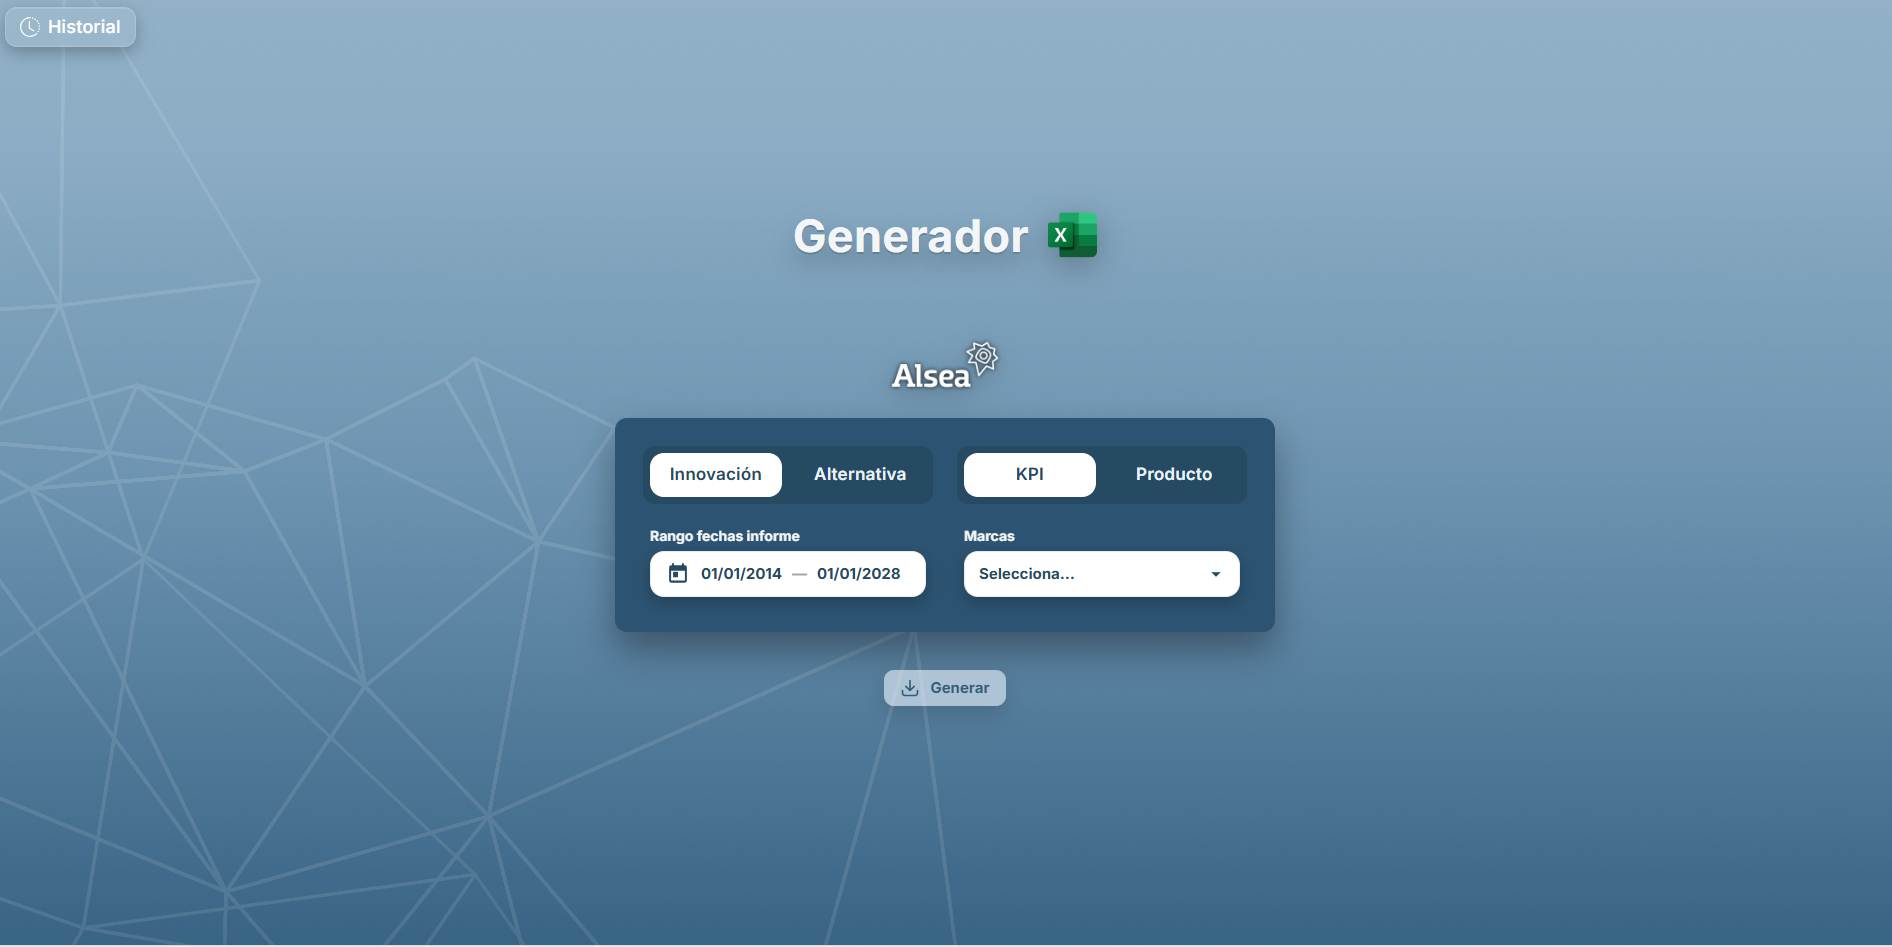
\includegraphics[width=0.9\textwidth]{generador.png}
  \caption{Interfaz principal del módulo de generación de informes.}
  \label{fig:generador}
\end{figure}

\subsection{Flujo de interacción}

El flujo de trabajo implementado en la página de generación garantiza una experiencia coherente y eficiente. El siguiente diagrama ilustra el proceso completo desde que el usuario accede a la página hasta que puede redescargar el informe desde el historial.

\begin{figure}[H]
  \centering
  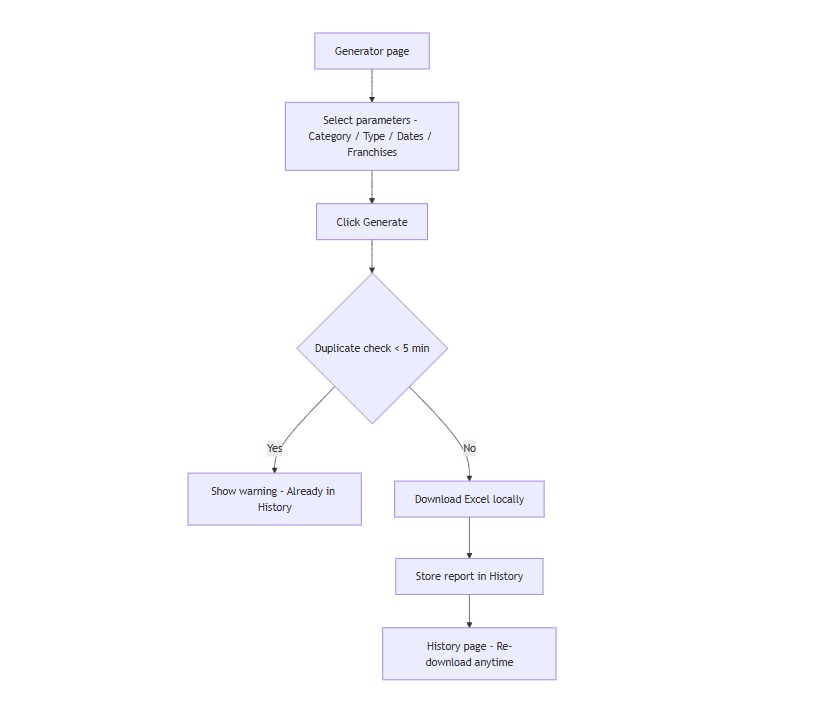
\includegraphics[width=0.7\textwidth]{img/diagrama_docu.jpg}
  \caption{Diagrama de flujo del proceso de generación de informes.}
  \label{fig:flujo-generador}
\end{figure}

Como se observa en la figura~\ref{fig:flujo-generador}, el proceso comienza cuando el usuario selecciona los parámetros del informe y pulsa el botón \textit{Generar}. En ese momento, el sistema comprueba si existe un informe idéntico generado en los últimos 5 minutos. Si se detecta un duplicado, el sistema consulta \texttt{/api/reports/latest} y muestra un aviso indicando si el informe ya está disponible o si la generación continúa en curso. En caso contrario, se inicia el job asíncrono y el frontend comienza a consultar periódicamente \texttt{/api/reports/latest}. Cuando la respuesta indica que el informe está listo, el cliente solicita su descarga automáticamente; en cualquier caso, el informe queda también disponible en Historial.

\section{Página de Historial}

La página de historial es una funcionalidad completamente nueva desarrollada en este proyecto. Antes de esta mejora, el sistema no contaba con ningún mecanismo para consultar informes previamente generados, obligando a los usuarios a regenerarlos cada vez que necesitaban acceder a información pasada.

\subsection{Funcionalidad}

\begin{itemize}
  \item Presenta una tabla con todos los informes generados.
  \item Cada fila incluye columnas de descarga, fecha de creación, tipo, categoría, franquicia(s), fechas y tamaño.
  \item Implementa paginación (\textit{5 anteriores} / \textit{5 siguientes}).
  \item Los informes se ordenan de los más recientes a los más antiguos.
  \item Permite la redescarga directa de cualquier informe almacenado.
\end{itemize}

\subsection{Diseño de la interfaz}

El diseño de la tabla de historial prioriza la claridad y la facilidad de uso. Cada informe muestra toda la información relevante de forma estructurada, permitiendo al usuario identificar rápidamente el documento que necesita. El botón de descarga en cada fila facilita el acceso inmediato al contenido sin necesidad de regenerar el informe.

\begin{figure}[H]
  \centering
  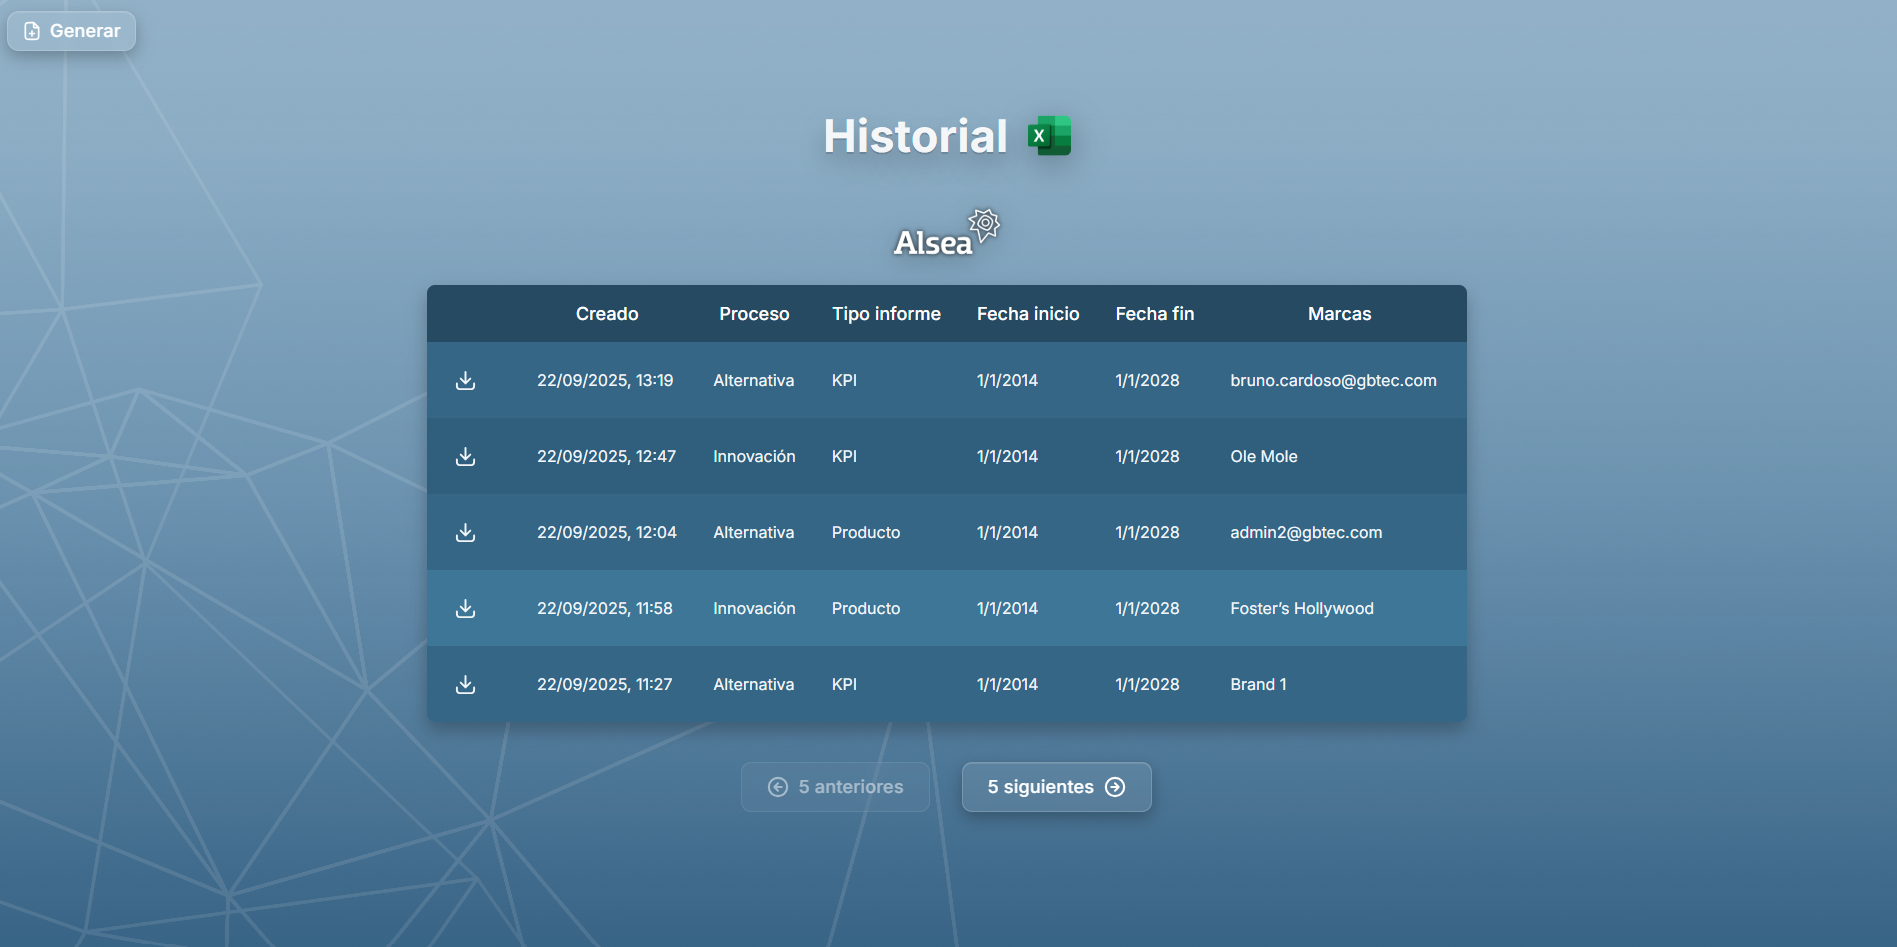
\includegraphics[width=0.9\textwidth]{historial.png}
  \caption{Vista de la página de historial de informes generados.}
  \label{fig:historial}
\end{figure}

\section{Release y publicación}

Una vez completado el desarrollo de las funcionalidades descritas, con las interfaces validadas y aprobadas por el equipo, y habiendo superado todas las pruebas de QA en el entorno de pruebas gestionado mediante AWX, el último paso consistía en preparar y publicar la nueva versión del Report Service siguiendo el proceso formal de release establecido por la empresa.\\

Este proceso seguía las convenciones de Gitflow y las políticas de versionado de GBTEC, garantizando la trazabilidad completa y minimizando riesgos de despliegue:

\begin{enumerate}
  \item \textbf{Creación de la rama release candidate (RC)}: desde la rama \texttt{development}, que contenía todos los cambios validados e integrados, se creaba una nueva rama \texttt{release/vX.Y.Z-rc} (por ejemplo, \texttt{release/v2.1.0-rc}). Esta rama servía como candidata para la release y permitía realizar ajustes finales sin bloquear el desarrollo de nuevas funcionalidades en \texttt{development}.
  
  \item \textbf{Version bump}: se actualizaban los números de versión en los archivos de configuración:
    \begin{itemize}
      \item Backend: actualización del elemento \texttt{<version>} en el archivo \texttt{pom.xml} de Maven.
    \end{itemize}
    Estos cambios se comprometían en la rama RC con un mensaje descriptivo (p. ej., \texttt{"chore: bump version to 2.1.0"}).
  
  \item \textbf{Builds y validaciones finales}: se ejecutaban los pipelines de GitHub Actions para compilar el proyecto completo, ejecutar todas las pruebas (unitarias e integradas) y verificar las métricas de calidad en SonarCloud. Se realizaba una última ronda de validaciones manuales en el entorno de QA para confirmar que no existían regresiones.
  
  \item \textbf{Merge a \texttt{main}}: se creaba un PR desde la rama RC hacia la rama \texttt{main}, que representaba el estado estable de producción. Tras la revisión final y aprobación por parte del equipo, se integraban los cambios mediante merge commit preservando el historial completo.
  
  \item \textbf{Creación del tag Git}: una vez completado el merge a \texttt{main}, se creaba un tag Git con el número de versión (e.g., \texttt{v2.1.0}) apuntando al commit de merge en la rama \texttt{main}. Este tag marcaba formalmente la versión publicable y permitía rastrear exactamente qué código se desplegó en producción.
  
  \item \textbf{Merge a \texttt{development}}: paralelamente, se integraban los cambios de la rama RC de vuelta a \texttt{development} para sincronizar cualquier ajuste realizado durante el proceso de release (como el version bump o correcciones de última hora), garantizando que \texttt{development} reflejara siempre el estado más actualizado.
  
  \item \textbf{Documentación}: se actualizaban los archivos README con notas de la release, se documentaban los cambios principales (changelog) y se comunicaba al cliente la disponibilidad de la nueva versión con sus mejoras y funcionalidades.
\end{enumerate}

Como parte del cierre del proyecto, también se revisó y amplió de forma exhaustiva la documentación de los repositorios frontend y backend. Antes de esta actualización, los README contenían información limitada sobre la configuración y la ejecución del servicio. La nueva documentación incorporó instrucciones de puesta en marcha, descripción de la configuración necesaria, dependencias, comandos habituales, estructura general y consideraciones para el despliegue, facilitando la incorporación de nuevos desarrolladores y el mantenimiento posterior.

Con este proceso, la nueva versión del Report Service quedó lista para su uso en producción, incorporando todas las mejoras de almacenamiento histórico, procesamiento asíncrono, control de duplicidad y experiencia de usuario modernizada.

%%%%%%%%%%%%%%%%%%%%%%%%%%%%%%%%%%%%%%%%%
 % Capítulo   8                         %
 %%%%%%%%%%%%%%%%%%%%%%%%%%%%%%%%%%%%%%%%

\chapter{Conclusión y trabajo futuro}

\section{Conclusiones}

Este Trabajo de Fin de Grado ha abordado la modernización del módulo
\textit{Report Service} integrado en la plataforma BIC para AESLA, dentro de
un proyecto desarrollado durante tres meses de prácticas en GBTEC Software
AG. Las tareas realizadas permitieron cubrir los principales objetivos
planteados al inicio del proyecto y ampliar tanto las capacidades funcionales
como la mantenibilidad del servicio. \\

Entre los principales resultados obtenidos destacan:

\begin{itemize}

  \item \textbf{Persistencia e historial de informes}: se incorporó un
  almacenamiento persistente en PostgreSQL, gestionado mediante migraciones
  Flyway. Los informes generados pueden conservarse junto con sus metadatos y
  recuperarse posteriormente desde la nueva página de historial, evitando la
  necesidad de regenerarlos para volver a acceder a ellos.

  \item \textbf{Procesamiento asíncrono}: la generación se integró con Spring
  Batch, desacoplando el procesamiento del ciclo principal de la petición
  HTTP. El frontend realiza un seguimiento periódico mediante
  \textit{polling}, permitiendo mantener la interfaz disponible mientras el
  informe se genera.

  \item \textbf{Control de duplicidad}: se incorporó una comprobación de
  solicitudes equivalentes dentro de una ventana temporal de cinco minutos,
  evitando iniciar una nueva generación cuando ya existe una solicitud
  reciente con los mismos parámetros.

  \item \textbf{Evolución de la interfaz}: se añadió una página específica de
  historial, nuevas validaciones y mensajes de estado asociados a la
  generación. Estas modificaciones proporcionan al usuario más información
  sobre el proceso y nuevas posibilidades de consulta y redescarga.

  \item \textbf{Mejora de las métricas de calidad}: la cobertura de código
  aumentó del 17.7\% al 25.7\%, superando el umbral mínimo del 20\% definido
  por la empresa. Paralelamente, la duplicación detectada por SonarCloud se
  redujo del 15.8\% al 10.0\%.

  \item \textbf{Gestión de dependencias y vulnerabilidades}: la
  estandarización del gestor de paquetes en Yarn y el uso controlado de
  \texttt{resolutions} permitieron reducir los avisos de seguridad asociados
  a las dependencias, aunque permanecieron tres vulnerabilidades menores
  vinculadas al \textit{tooling} de la versión utilizada de Angular.

\end{itemize}

Desde el punto de vista formativo, el proyecto permitió trabajar sobre una
aplicación empresarial existente, donde las decisiones debían considerar no
solo la implementación de nuevas funcionalidades, sino también la
compatibilidad con código previo, la calidad, las pruebas, la seguridad y el
proceso de despliegue. El uso de Jira, Git, Pull Requests, revisión de código,
pipelines de integración continua y entornos de QA proporcionó una visión
práctica del ciclo de desarrollo de software en un entorno profesional. \\

En conjunto, la solución desarrollada amplía de forma significativa las
capacidades del Report Service respecto a su estado inicial y establece una
base más mantenible para futuras evoluciones. Los resultados obtenidos
responden a los objetivos funcionales definidos para el proyecto, aunque
existen limitaciones y líneas de mejora que se detallan a continuación. \\ 

\section{Limitaciones}

Aunque los objetivos principales del proyecto fueron alcanzados, el alcance
temporal y el contexto de desarrollo condicionaron algunas de las decisiones
adoptadas. Las principales limitaciones identificadas son las siguientes:

\begin{itemize}

  \item \textbf{Ausencia de pruebas formales de carga}: se validó
  funcionalmente la generación asíncrona y la ejecución de los principales
  flujos, pero no se realizó un estudio específico de rendimiento bajo
  concurrencia elevada. Por tanto, no se dispone de métricas que permitan
  cuantificar el comportamiento del sistema ante un número elevado de
  generaciones simultáneas.

  \item \textbf{Versión del frontend}: el proyecto permanece sobre Angular 15.
  Aunque se mitigaron gran parte de los avisos de seguridad asociados a las
  dependencias, quedaron tres vulnerabilidades menores relacionadas con el
  \textit{tooling} de esta versión.

  \item \textbf{Ausencia de una política de retención}: los informes
  almacenados permanecen actualmente en la base de datos sin un mecanismo
  automático de eliminación o una política de conservación configurable.

  \item \textbf{Seguimiento de la generación}: el estado se consulta mediante
  \textit{polling} periódico. Aunque este mecanismo permite detectar cuándo el
  informe está disponible, no proporciona un porcentaje de progreso ni
  información detallada sobre las distintas etapas internas de generación.

  \item \textbf{Evaluación de usabilidad}: las interfaces fueron validadas
  funcionalmente dentro del proceso de QA, pero no se realizó un estudio
  formal de usabilidad con usuarios finales ni se recopilaron métricas
  cuantitativas de experiencia de usuario.

\end{itemize}

Estas limitaciones no impiden el funcionamiento de las funcionalidades
desarrolladas, pero delimitan el alcance de las conclusiones que pueden
extraerse y permiten identificar posibles líneas de evolución del sistema. \\

\section{Posibles ampliaciones futuras}

Aunque el proyecto ha logrado cumplir con los objetivos planteados, existen diversas líneas de trabajo que podrían abordarse en el futuro para seguir mejorando el Report Service. Estas ampliaciones se han identificado durante el desarrollo del proyecto y representan oportunidades para aumentar la funcionalidad, seguridad y usabilidad del sistema.

\subsection{Actualización de la versión de Angular}

Como se indicó en el apartado de vulnerabilidades y en las limitaciones del
proyecto, una de las principales mejoras pendientes consiste en migrar
Angular 15 a una versión posterior compatible con el resto del stack y que
disponga de soporte vigente. \\

Esta actualización permitiría:

\begin{itemize}

  \item Reevaluar el árbol completo de dependencias del frontend.

  \item Reducir o eliminar, cuando sea posible, el bloque
  \texttt{resolutions} utilizado actualmente en
  \texttt{package.json}.

  \item Analizar nuevamente las vulnerabilidades residuales y utilizar
  versiones corregidas de las dependencias cuando estén disponibles.

  \item Beneficiarse de las mejoras introducidas en versiones posteriores del
  framework y de Angular Material.

  \item Reducir las incompatibilidades entre dependencias heredadas del
  proyecto.

\end{itemize}

La migración debería realizarse de forma progresiva, siguiendo las guías
oficiales de actualización y validando el comportamiento de la aplicación
tras cada cambio de versión. Debido a las posibles incompatibilidades entre
dependencias, sería necesario acompañar la actualización de pruebas
funcionales y de regresión. \\

\subsection{Mejoras en la gestión del historial}

Una de las funcionalidades más solicitadas para futuras versiones es la ampliación de las capacidades de gestión del historial de informes. Específicamente, se ha identificado la necesidad de implementar:

\subsubsection{Eliminación de informes}

Actualmente, todos los informes generados se almacenan indefinidamente en la base de datos, sin una política de retención explícita. Sería deseable permitir a los usuarios eliminar informes que ya no necesiten, liberando espacio de almacenamiento y facilitando la gestión del historial.\\

El diseño preliminar de esta funcionalidad incluiría:

\begin{figure}[H]
  \centering
  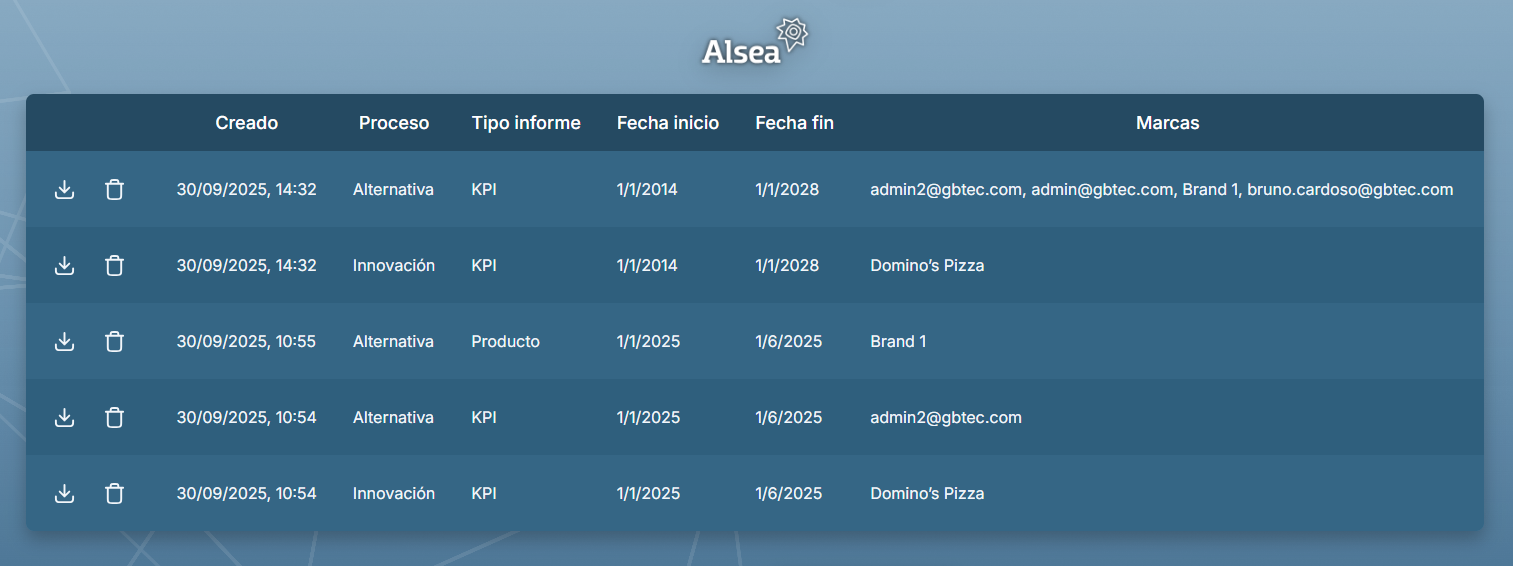
\includegraphics[width=0.9\textwidth]{img/historial_borrar.png}
  \caption{Mockup de la interfaz de historial con funcionalidad de eliminación de informes.}
  \label{fig:historial-borrar}
\end{figure}

Como se observa en la figura~\ref{fig:historial-borrar}, se añadiría una columna adicional con botones de eliminación para cada informe. Al pulsar el botón de borrar, aparecería un diálogo de confirmación para evitar eliminaciones accidentales.

\begin{figure}[H]
  \centering
  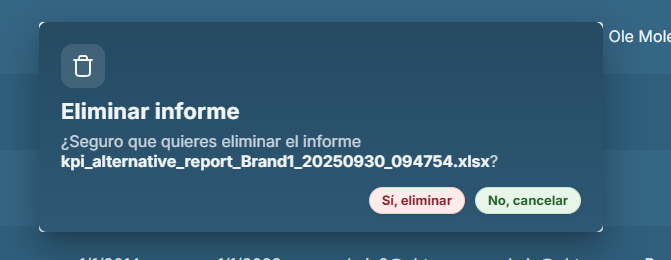
\includegraphics[width=0.6\textwidth]{img/emergente_borrar.png}
  \caption{Diálogo de confirmación para la eliminación de informes.}
  \label{fig:emergente-borrar}
\end{figure}

La figura~\ref{fig:emergente-borrar} muestra el diseño del diálogo de confirmación que solicitaría al usuario verificar la acción antes de eliminar permanentemente un informe del sistema.

\subsubsection{Otras mejoras planificadas para el historial}

Además de la funcionalidad de eliminación, se han identificado otras mejoras deseables:

\begin{itemize}
    \item \textbf{Selección múltiple}: implementar checkboxes para seleccionar varios informes y realizar acciones en lote (eliminar múltiples informes, descargar varios informes simultáneamente).
    \item \textbf{Filtros avanzados}: añadir filtros por categoría, tipo, franquicia, rango de fechas, etc., para facilitar la búsqueda de informes específicos en historiales extensos.
    \item \textbf{Ordenación personalizable}: permitir ordenar la tabla por diferentes columnas (fecha, tamaño, tipo, categoría).
    \item \textbf{Exportación del listado}: posibilidad de exportar el listado del historial a CSV o Excel para auditorías o análisis externos.
\end{itemize}

\subsection{Refactorización adicional del código backend}

Aunque durante el proyecto se realizaron importantes tareas de refactorización que mejoraron las métricas de calidad del código, siempre existe margen de mejora. Las áreas identificadas para futuras mejoras incluyen:

\begin{itemize}
    \item Mayor modularización de utilidades comunes.
    \item Ampliación de la cobertura de pruebas unitarias e integradas.
    \item Optimización de consultas a la base de datos.
    \item Implementación de patrones de diseño adicionales para mejorar la mantenibilidad.
\end{itemize}

\subsection{Funcionalidades avanzadas}

Mirando más allá de las mejoras inmediatas, se podrían considerar funcionalidades más ambiciosas:

\begin{itemize}
    \item \textbf{Programación de informes}: permitir a los usuarios programar la generación automática de informes periódicos.
    \item \textbf{Notificaciones}: enviar notificaciones cuando un informe esté listo.
    \item \textbf{Plantillas personalizables}: permitir a los usuarios definir plantillas de informe con métricas específicas.
    \item \textbf{Dashboard analítico}: crear visualizaciones interactivas de las métricas de los informes sin necesidad de descargar Excel.
    \item \textbf{Control de acceso granular}: implementar permisos específicos por usuario o rol para la generación y consulta de informes.
\end{itemize}

Estas ampliaciones futuras representan oportunidades para seguir evolucionando el Report Service hacia una herramienta cada vez más completa y alineada con las necesidades cambiantes de AESLA.


 %%%%%%%%%%%%%%%%%%%%%%%%%%%%%%%%%%%%%%%%
 % Apéndices, glosarios e bibliografía  %
 %%%%%%%%%%%%%%%%%%%%%%%%%%%%%%%%%%%%%%%%

 \appendix
 \appendixpage
 %%%%%%%%%%%%%%%%%%%%%%%%%%%%%%%%%%%%%%%%%
% Apéndice: Evidencias técnicas         %
%%%%%%%%%%%%%%%%%%%%%%%%%%%%%%%%%%%%%%%%%

\chapter{Evidencias técnicas}
\label{ap:evidencias-tecnicas}


%%%%%%%%%%%%%%%%%%%%%%%%%%%%%%%%%%%%%%%%%
% Arquitectura detallada                %
%%%%%%%%%%%%%%%%%%%%%%%%%%%%%%%%%%%%%%%%%

\section{Arquitectura detallada}
\label{ap:arquitectura-detallada}

La figura~\ref{fig:arquitectura-detallada} amplía la representación
simplificada presentada en el capítulo~5 e incorpora los principales
componentes internos del frontend y del backend, el procesamiento asíncrono
mediante Spring Batch, las fuentes de datos y los elementos de
infraestructura utilizados durante el despliegue.

\begin{figure}[H]
  \centering
  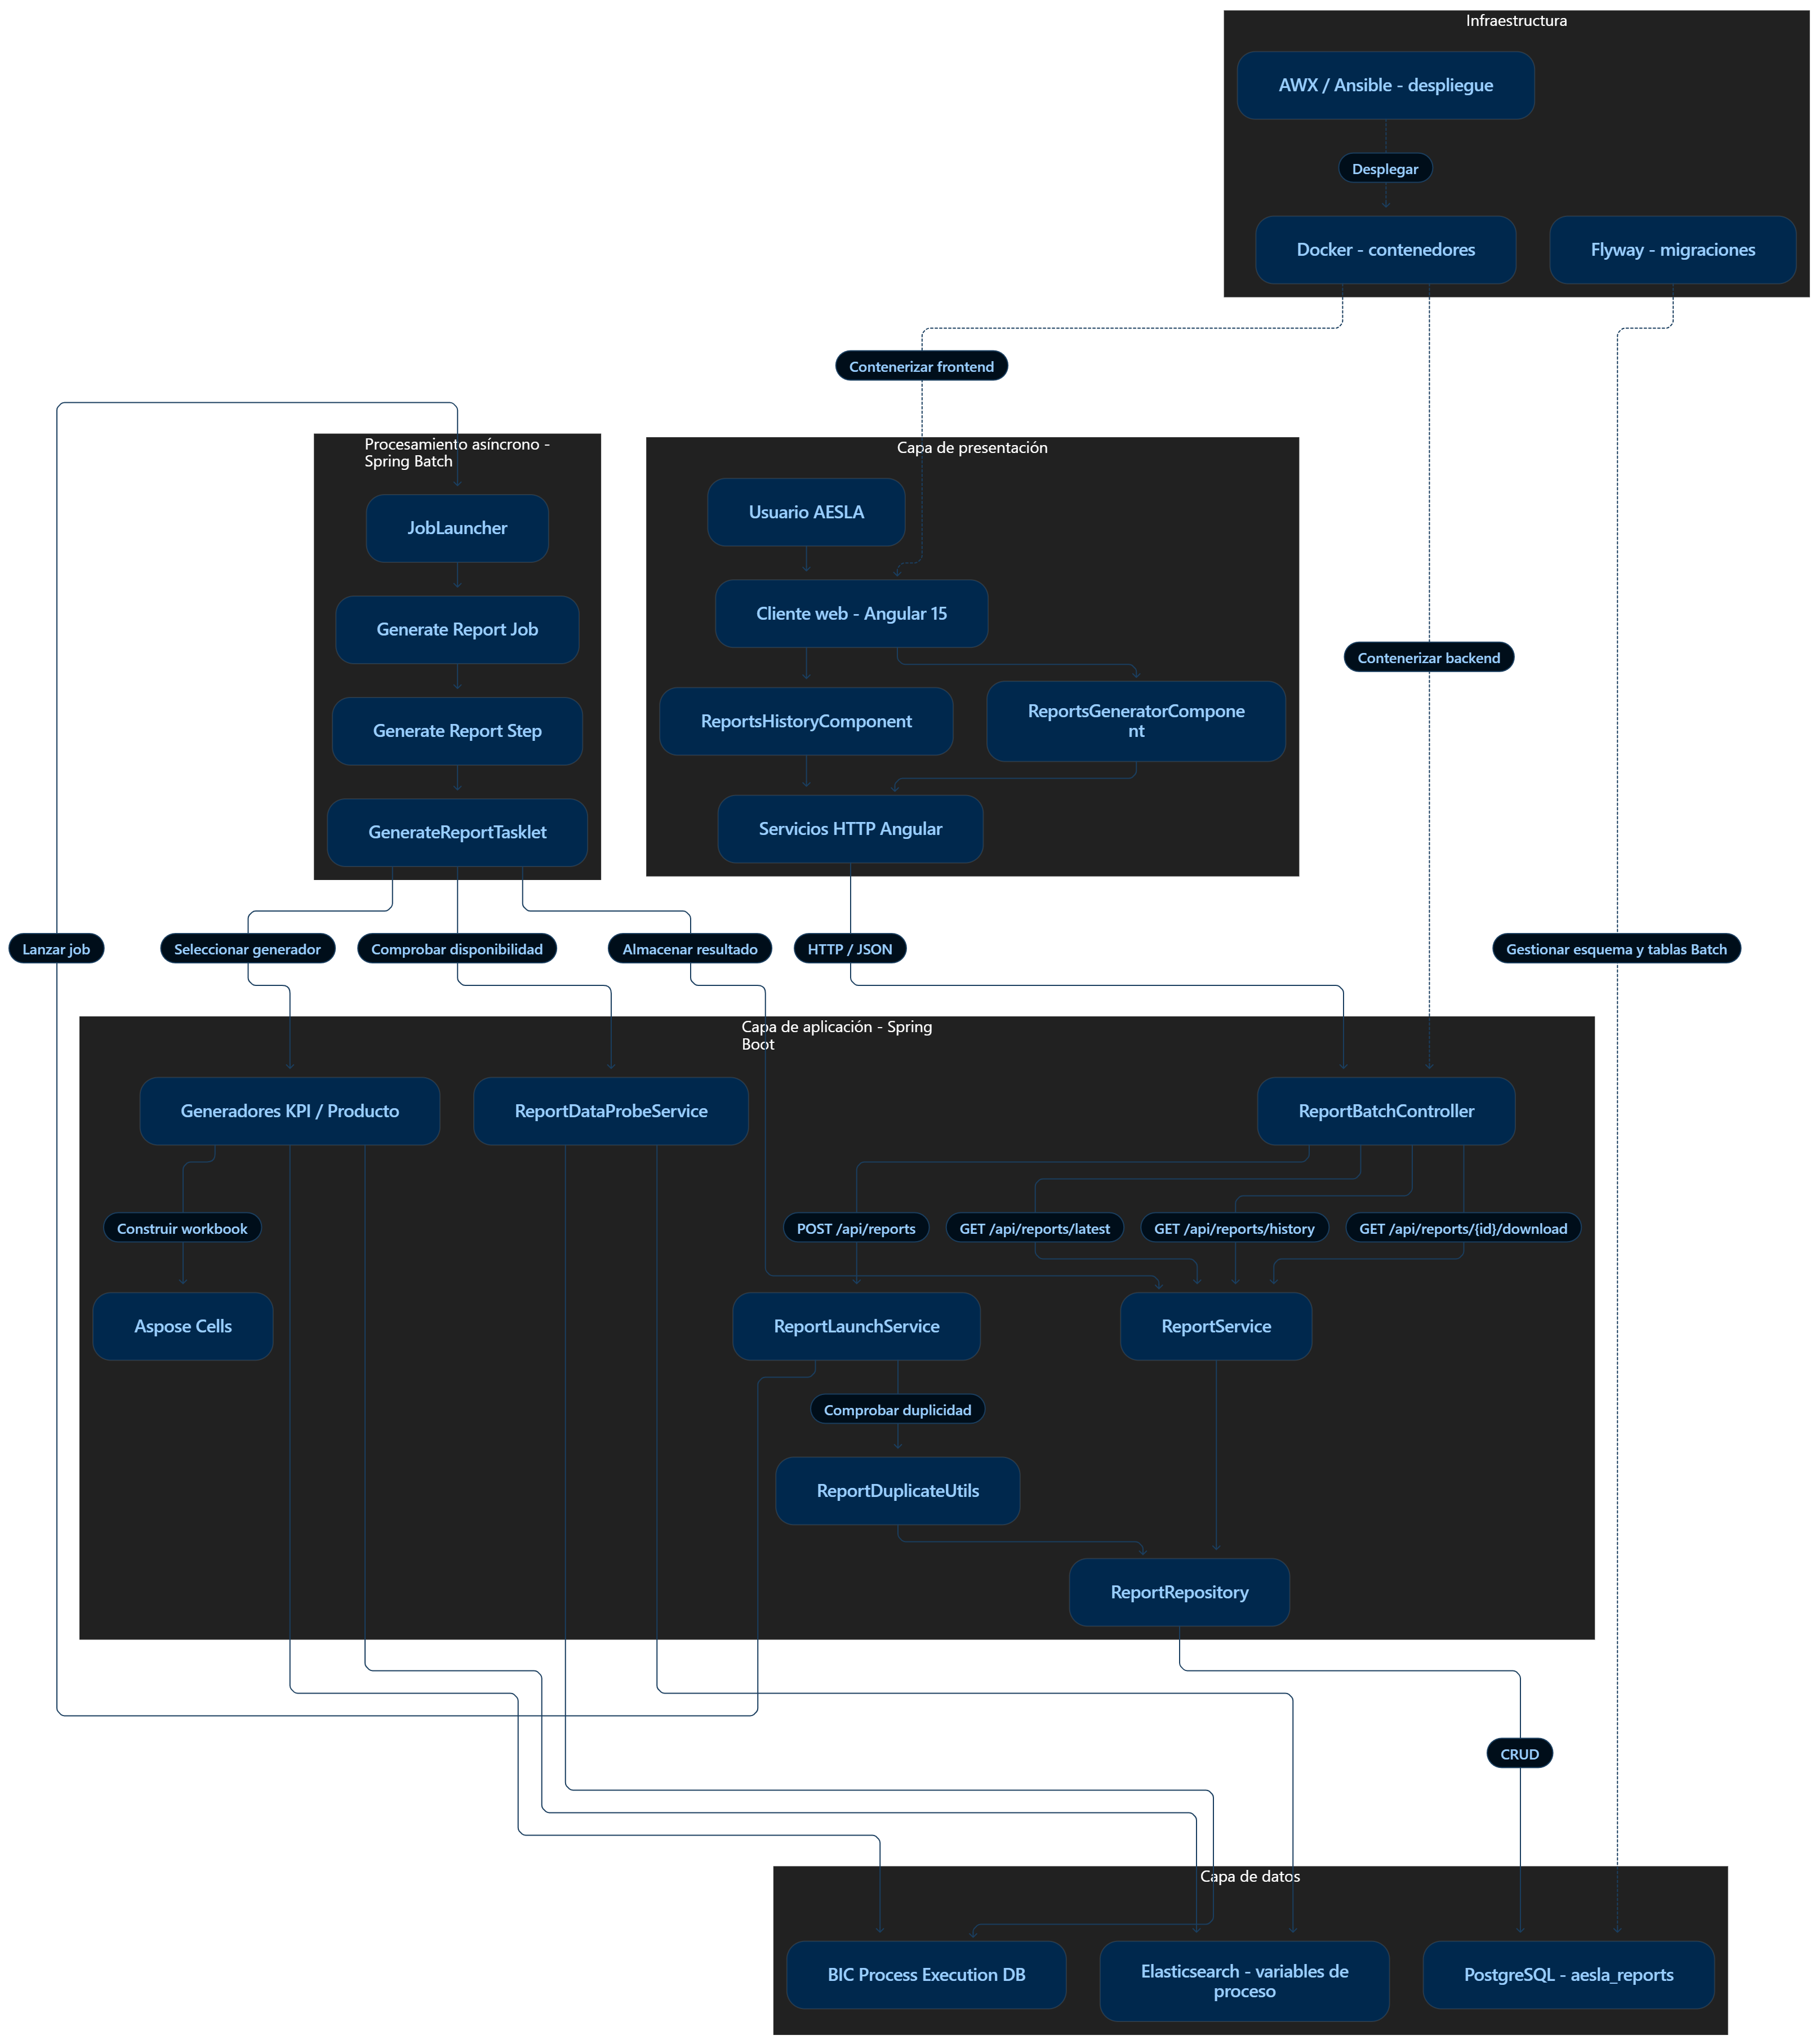
\includegraphics[width=\textwidth]{img/arquitectura_detallada.png}
  \caption{Arquitectura detallada del Report Service. Fuente: elaboración propia.}
  \label{fig:arquitectura-detallada}
\end{figure}

En la capa de presentación, el usuario interactúa con los componentes Angular
de generación e historial, que centralizan sus comunicaciones con el backend
a través de servicios HTTP. El punto de entrada en la capa de aplicación es
\texttt{ReportBatchController}, encargado de exponer las operaciones REST
utilizadas por el cliente.

Para una nueva generación, el controlador delega en
\texttt{ReportLaunchService}, que realiza la comprobación previa de
duplicidad antes de iniciar el job de Spring Batch. El procesamiento
asíncrono se articula mediante \texttt{JobLauncher}, un job, un step y
\texttt{GenerateReportTasklet}. Durante su ejecución se comprueba la
disponibilidad de datos mediante \texttt{ReportDataProbeService} y se
selecciona la lógica de generación correspondiente al tipo y categoría de
informe.

Los datos utilizados proceden de BIC Process Execution y Elasticsearch,
mientras que Aspose Cells proporciona las operaciones necesarias para la
construcción de los libros Excel. Finalmente, \texttt{ReportService}
centraliza el almacenamiento del resultado y utiliza
\texttt{ReportRepository} para persistir el contenido y sus metadatos en el
esquema \texttt{aesla\_reports} de PostgreSQL.

La infraestructura complementaria incluye Flyway para gestionar las
migraciones de base de datos, Docker para la contenerización de los servicios
y AWX/Ansible para automatizar su despliegue en los diferentes entornos.


%%%%%%%%%%%%%%%%%%%%%%%%%%%%%%%%%%%%%%%%%
% Evidencias de calidad de código       %
%%%%%%%%%%%%%%%%%%%%%%%%%%%%%%%%%%%%%%%%%

\section{Evidencias de calidad de código}
\label{ap:evidencias-sonar}

Las siguientes figuras recogen las capturas de SonarCloud utilizadas como
evidencia de las métricas de cobertura y duplicación presentadas en el
capítulo~6. En el cuerpo principal de la memoria se muestran únicamente los
valores iniciales y finales, mientras que las capturas completas se trasladan
a este apéndice para facilitar su consulta sin sobrecargar el capítulo de
implementación y pruebas.

\begin{figure}[H]
  \centering
  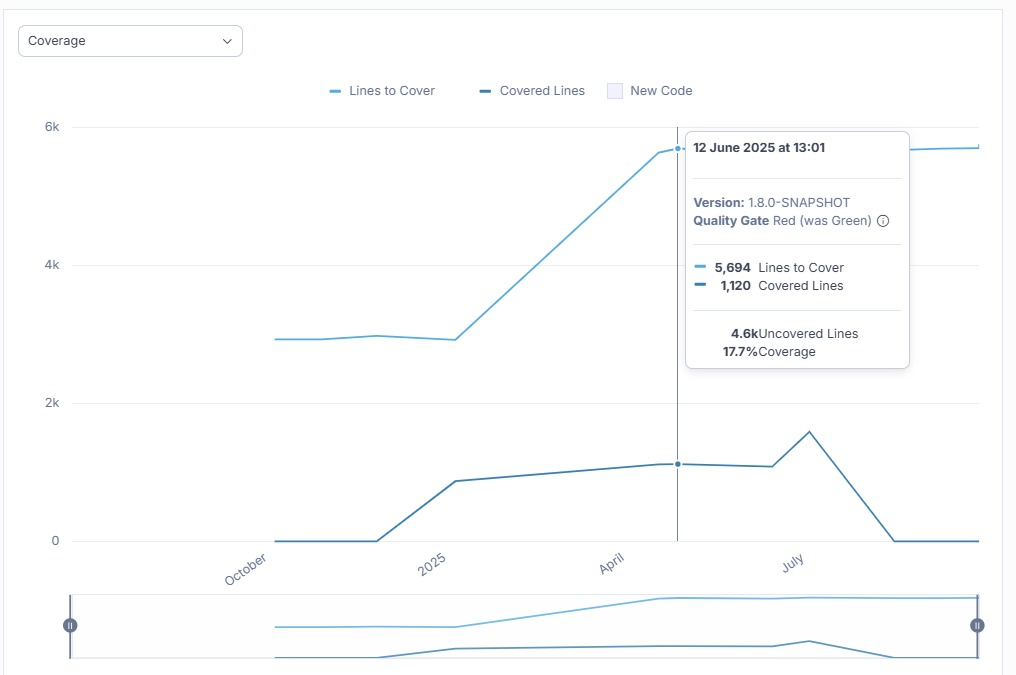
\includegraphics[width=0.85\textwidth]{img/coverage_before.jpeg}
  \caption{Captura de SonarCloud correspondiente a la cobertura inicial del proyecto: 17.7\%.}
  \label{fig:coverage-before}
\end{figure}

\begin{figure}[H]
  \centering
  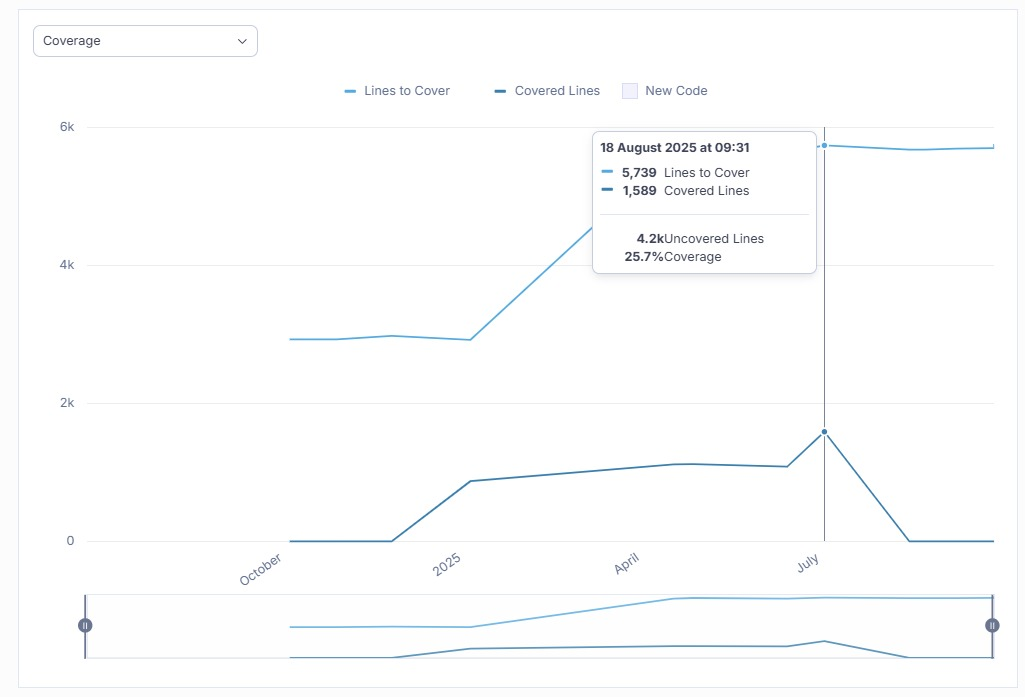
\includegraphics[width=0.85\textwidth]{img/coverage_after.jpeg}
  \caption{Captura de SonarCloud correspondiente a la cobertura final del proyecto: 25.7\%.}
  \label{fig:coverage-after}
\end{figure}

\begin{figure}[H]
  \centering
  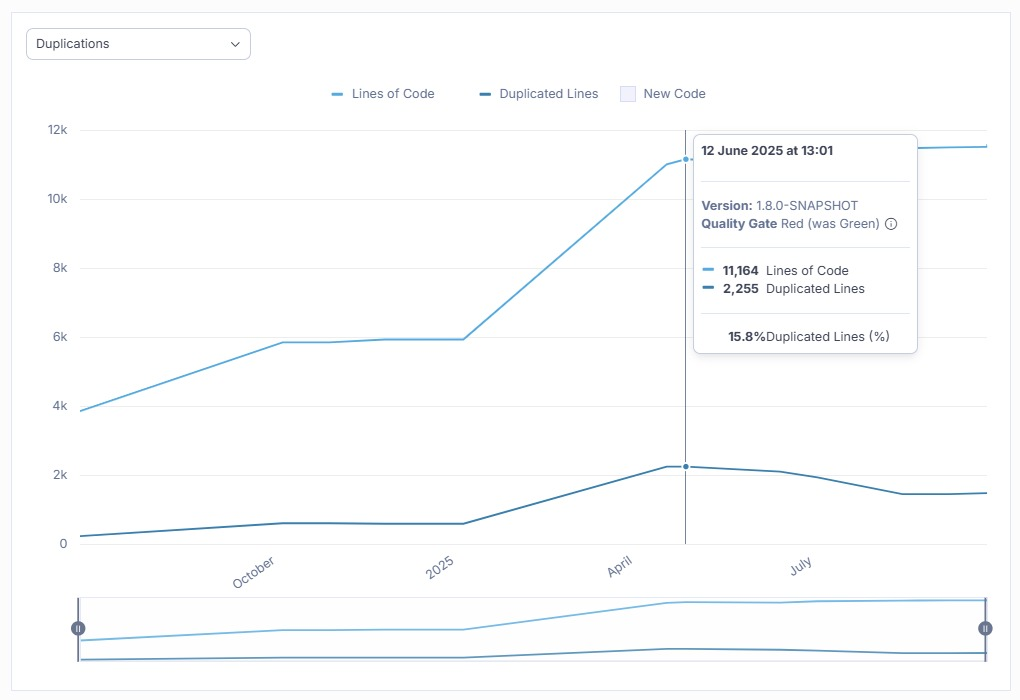
\includegraphics[width=0.85\textwidth]{img/duplications_before.jpeg}
  \caption{Captura de SonarCloud correspondiente a la duplicación inicial del proyecto: 15.8\%.}
  \label{fig:duplications-before}
\end{figure}

\begin{figure}[H]
  \centering
  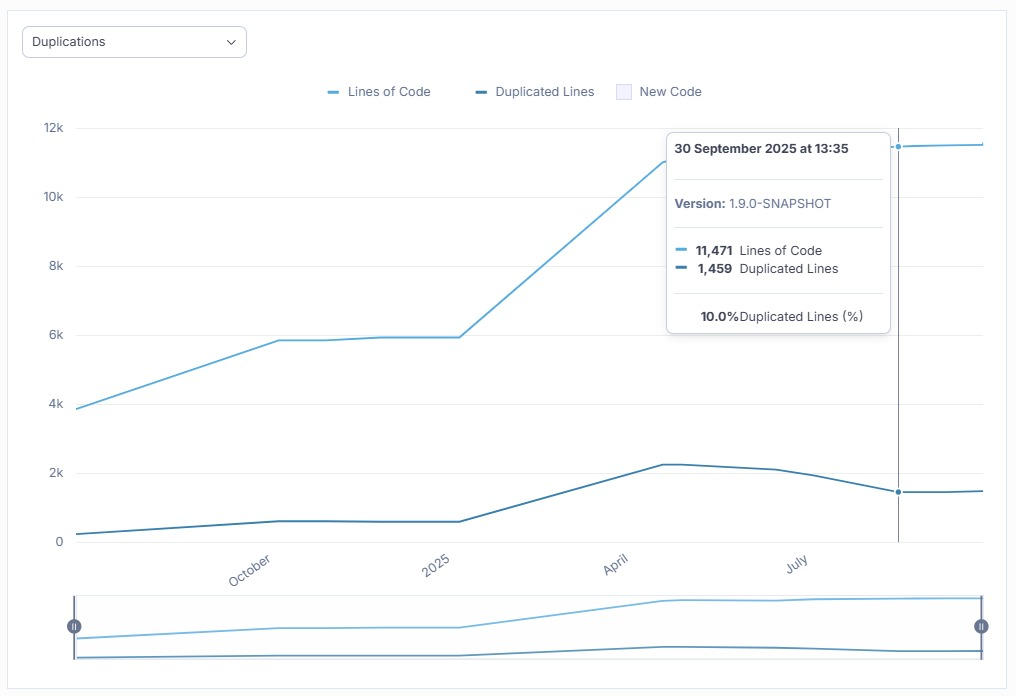
\includegraphics[width=0.85\textwidth]{img/duplications_after.jpeg}
  \caption{Captura de SonarCloud correspondiente a la duplicación final del proyecto: 10.0\%.}
  \label{fig:duplications-after}
\end{figure}
%\include{anexos/...}

 \printglossary[type=\acronymtype,title=\nomeglosarioacronimos]
 \printglossary[title=\nomeglosariotermos]

 \bibliographystyle{IEEEtranN}
 \bibliography{\bibconfig,bibliografia/bibliografia}
 \clearpage
 
\end{document}

%%%%%%%%%%%%%%%%%%%%%%%%%%%%%%%%%%%%%%%%%%%%%%%%%%%%%%%%%%%%%%%%%%%%%%%%%%%%%%%%
